%%%%%%%%%%%%%%%%%%%%%%%%%%%%%%%%%%%%%%%%%
% Beamer Presentation
% LaTeX Template
% Version 1.0 (10/11/12)
%
% This template has been downloaded from:
% http://www.LaTeXTemplates.com
%
% License:
% CC BY-NC-SA 3.0 (http://creativecommons.org/licenses/by-nc-sa/3.0/)
%
%%%%%%%%%%%%%%%%%%%%%%%%%%%%%%%%%%%%%%%%%

%----------------------------------------------------------------------------------------
%	PACKAGES AND THEMES
%----------------------------------------------------------------------------------------

\documentclass[aspectratio=169, 8pt]{beamer}

\mode<presentation> {

% The Beamer class comes with a number of default slide themes
% which change the colors and layouts of slides. Below this is a list
% of all the themes, uncomment each in turn to see what they look like.

%\usetheme{default}
%\usetheme{AnnArbor}
%\usetheme{Antibes}
%\usetheme{Bergen}
%\usetheme{Berkeley}
%\usetheme{Berlin}
%\usetheme{Boadilla}
%\usetheme{CambridgeUS}
%\usetheme{Copenhagen}
\usetheme{Darmstadt}
%\usetheme{Dresden}
%\usetheme{Frankfurt}
%\usetheme{Goettingen}
% \usetheme{Hannover}
%\usetheme{Ilmenau}
%\usetheme{JuanLesPins}
% \usetheme{Luebeck}
% \usetheme{Madrid}
%\usetheme{Malmoe}
%\usetheme{Marburg}
%\usetheme{Montpellier}
%\usetheme{PaloAlto}
%\usetheme{Pittsburgh}
%\usetheme{Rochester}
%\usetheme{Singapore}
%\usetheme{Szeged}
%\usetheme{Warsaw}

% As well as themes, the Beamer class has a number of color themes
% for any slide theme. Uncomment each of these in turn to see how it
% changes the colors of your current slide theme.

% \usecolortheme{albatross}
%\usecolortheme{beaver}
%\usecolortheme{beetle}
% \usecolortheme{crane}
% \usecolortheme{dolphin}
% \usecolortheme{dove}
% \usecolortheme{fly}
%\usecolortheme{lily}
%\usecolortheme{orchid}
%\usecolortheme{rose}
% \usecolortheme{seagull}
% \usecolortheme{seahorse}
\usecolortheme{whale}
%\usecolortheme{wolverine}

%\setbeamertemplate{footline} % To remove the footer line in all slides uncomment this line
%\setbeamertemplate{footline}[page number] % To replace the footer line in all slides with a simple slide count uncomment this line

%\setbeamertemplate{navigation symbols}{} % To remove the navigation symbols from the bottom of all slides uncomment this line
}

\usepackage{graphicx}
\usepackage{colortbl}
\usepackage{multirow}
\usepackage{graphicx}
\usepackage{tabularx}
\usepackage{xurl}
\usepackage{color}
\usepackage{graphicx} % Allows including images
\usepackage{booktabs} % Allows the use of \toprule, \midrule and \bottomrule in tables

%----------------------------------------------------------------------------------------
%	TITLE PAGE
%----------------------------------------------------------------------------------------

\title[Short Title]{Applied GPS Spoofing Detection on Drones} % The short title appears at the bottom of every slide, the full title is only on the title page

\author{Xiaohan Wang, Chengqi Liu, Guangyu Li} % Your name
\institute[TU Eindhoven] % Your institution as it will appear on the bottom of every slide, may be shorthand to save space
{
TU Eindhoven \\ % Your institution for the title page
\medskip% Your email address
}
\date{\today} % Date, can be changed to a custom date



\begin{document}

\begin{frame}
\titlepage % Print the title page as the first slide
\end{frame}

\begin{frame}
\frametitle{Overview} % Table of contents slide, comment this block out to remove it
\tableofcontents % Throughout your presentation, if you choose to use \section{} and \subsection{} commands, these will automatically be printed on this slide as an overview of your presentation
\end{frame}

%----------------------------------------------------------------------------------------
%	PRESENTATION SLIDES
%----------------------------------------------------------------------------------------






%------------------------------------------------
\section{Introduction} % Sections can be created in order to organize your presentation into discrete blocks, all sections and subsections are automatically printed in the table of contents as an overview of the talk
%------------------------------------------------

\subsection{Overview} 

\begin{frame}{UAVs/Drones \& The Threats of GPS Spoofing Attacks}

\begin{columns}
    \begin{column}{0.5 \linewidth}
        \begin{itemize}
            \item \large{Unmanned Aerial Vehicle (UAV) or "Drones"}
            \item The Threats of GPS Spoofing Attacks
            \item The importance of anti-attack spoofing detection methods
        \end{itemize}
    \end{column}

    \begin{column}{0.5 \linewidth}

        \begin{figure}
            \centering
            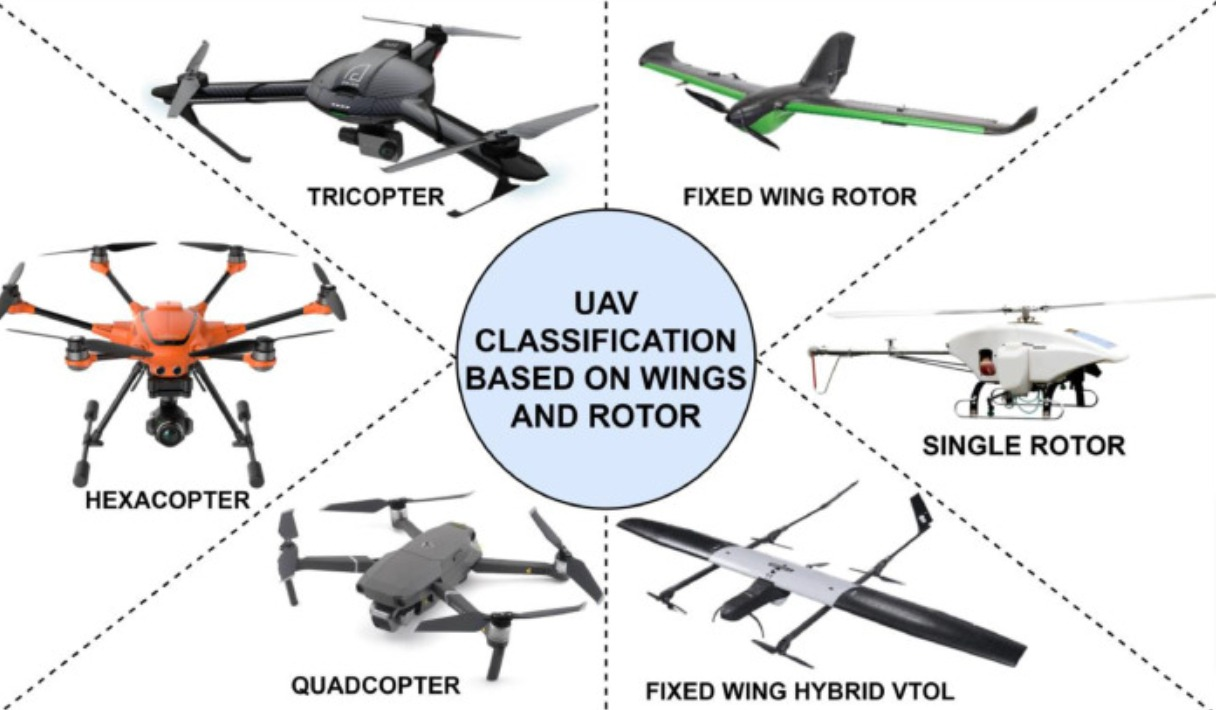
\includegraphics[width = 0.5\linewidth]{images/Detail-Guide-about-UAV-Technology-Supporting-Aerial-Task-Operations-Google-Docs.jpeg}
            \caption{Various kinds of UAVs}
            \label{fig:enter-label}
        \end{figure}
        
        \begin{figure}
            \centering
            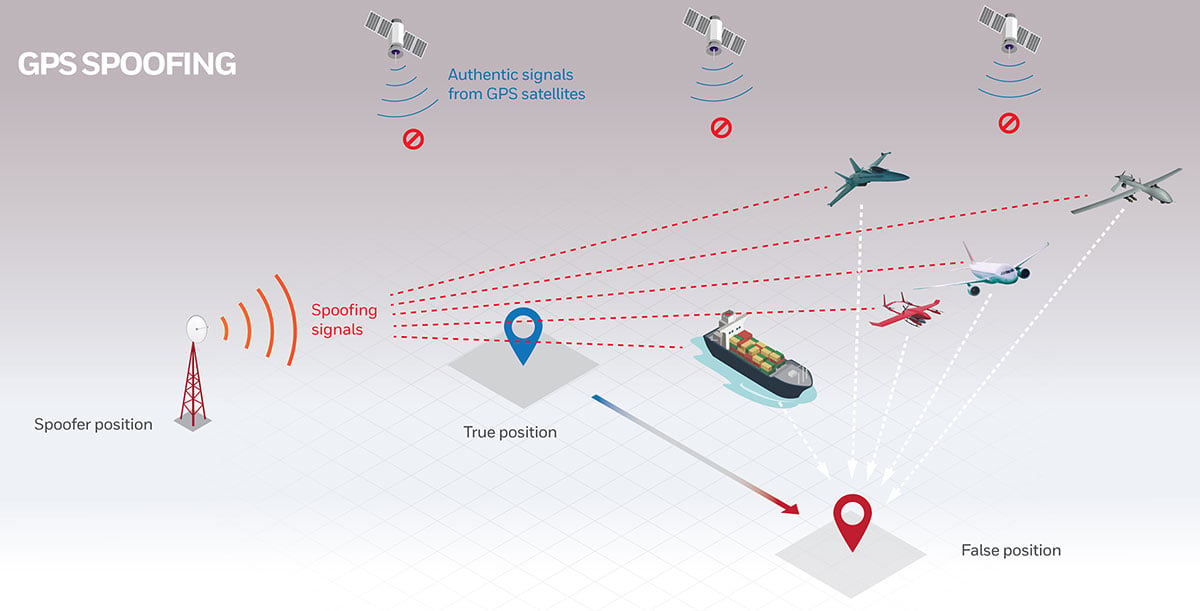
\includegraphics[width = 0.7\linewidth]{images/spoofing-Honeywell-alternative-navigation-W.jpg}
            \caption{GPS spoofing}
            \label{fig:enter-label}
        \end{figure}
        
    \end{column}
\end{columns}

\end{frame}

%------------------------------------------------
\subsection{Contributions}
\begin{frame}
\frametitle{Our Contributions}

\large
\begin{itemize}
    
    \item Literature review on GPS spoofing and spoofing detection methods.
    % \begin{itemize}
    %     \item 
    % \end{itemize}
    \item Selecting models for this comparative study.
    \item Carrying out experiments for selected methods on a single dataset.
    \begin{itemize}
        \item This is a nontrivial task, given the varying scenarios and model inputs across the academic papers in this field.
    \end{itemize}
    \item Reflecting on the pros and cons of the select methods.
\end{itemize}

\end{frame}

%------------------------------------------------

%------------------------------------------------

% \begin{frame}
% \frametitle{Blocks of Highlighted Text}
% \begin{block}{Block 1}
% Lorem ipsum dolor sit amet, consectetur adipiscing elit. Integer lectus nisl, ultricies in feugiat rutrum, porttitor sit amet augue. Aliquam ut tortor mauris. Sed volutpat ante purus, quis accumsan dolor.
% \end{block}


% \begin{block}{Block 3}
% Suspendisse tincidunt sagittis gravida. Curabitur condimentum, enim sed venenatis rutrum, ipsum neque consectetur orci, sed blandit justo nisi ac lacus.
% \end{block}
% \end{frame}

%------------------------------------------------

% \begin{frame}
% \frametitle{Multiple Columns}
% \begin{columns}[c] % The "c" option specifies centered vertical alignment while the "t" option is used for top vertical alignment

% \column{.45\textwidth} % Left column and width
% \textbf{Heading}
% \begin{enumerate}
% \item Statement
% \item Explanation
% \item Example
% \end{enumerate}

% \column{.5\textwidth} % Right column and width
% Lorem ipsum dolor sit amet, consectetur adipiscing elit. Integer lectus nisl, ultricies in feugiat rutrum, porttitor sit amet augue. Aliquam ut tortor mauris. Sed volutpat ante purus, quis accumsan dolor.

% \end{columns}
% \end{frame}














%------------------------------------------------
\section{Background \& Literature Review}
%------------------------------------------------

\subsection{UAVs and GPS}

\begin{frame}{UAVs and GPS}

\begin{columns}

\column{.45\textwidth} % Left column and width
\begin{itemize}
    \item Global navigation satellite system (GNSS) supports the navigation of a UAV.
    \item GNSS
    \begin{itemize}
        \item an umberella term for all satellite-based
navigation networks worldwide including the Global Positioning System (GPS).
    \end{itemize}
    \item GPS Signals
    \begin{itemize}
        \item Military GPS Signal: Encrypted. 
        \item Civilian GPS Signal: Not encrypted. Uses publicly available codes.
    \end{itemize}
    \item Other device on UAVs:
    \begin{itemize}
        \item GNSS/GPS receiver: Positional data
        \item Other sensory devices: IMU, RSS, etc: angular velocity, acceleration, etc.
    \end{itemize}
    
\end{itemize}

\column{.5\textwidth} % Right column and width

\begin{figure}
    \centering
    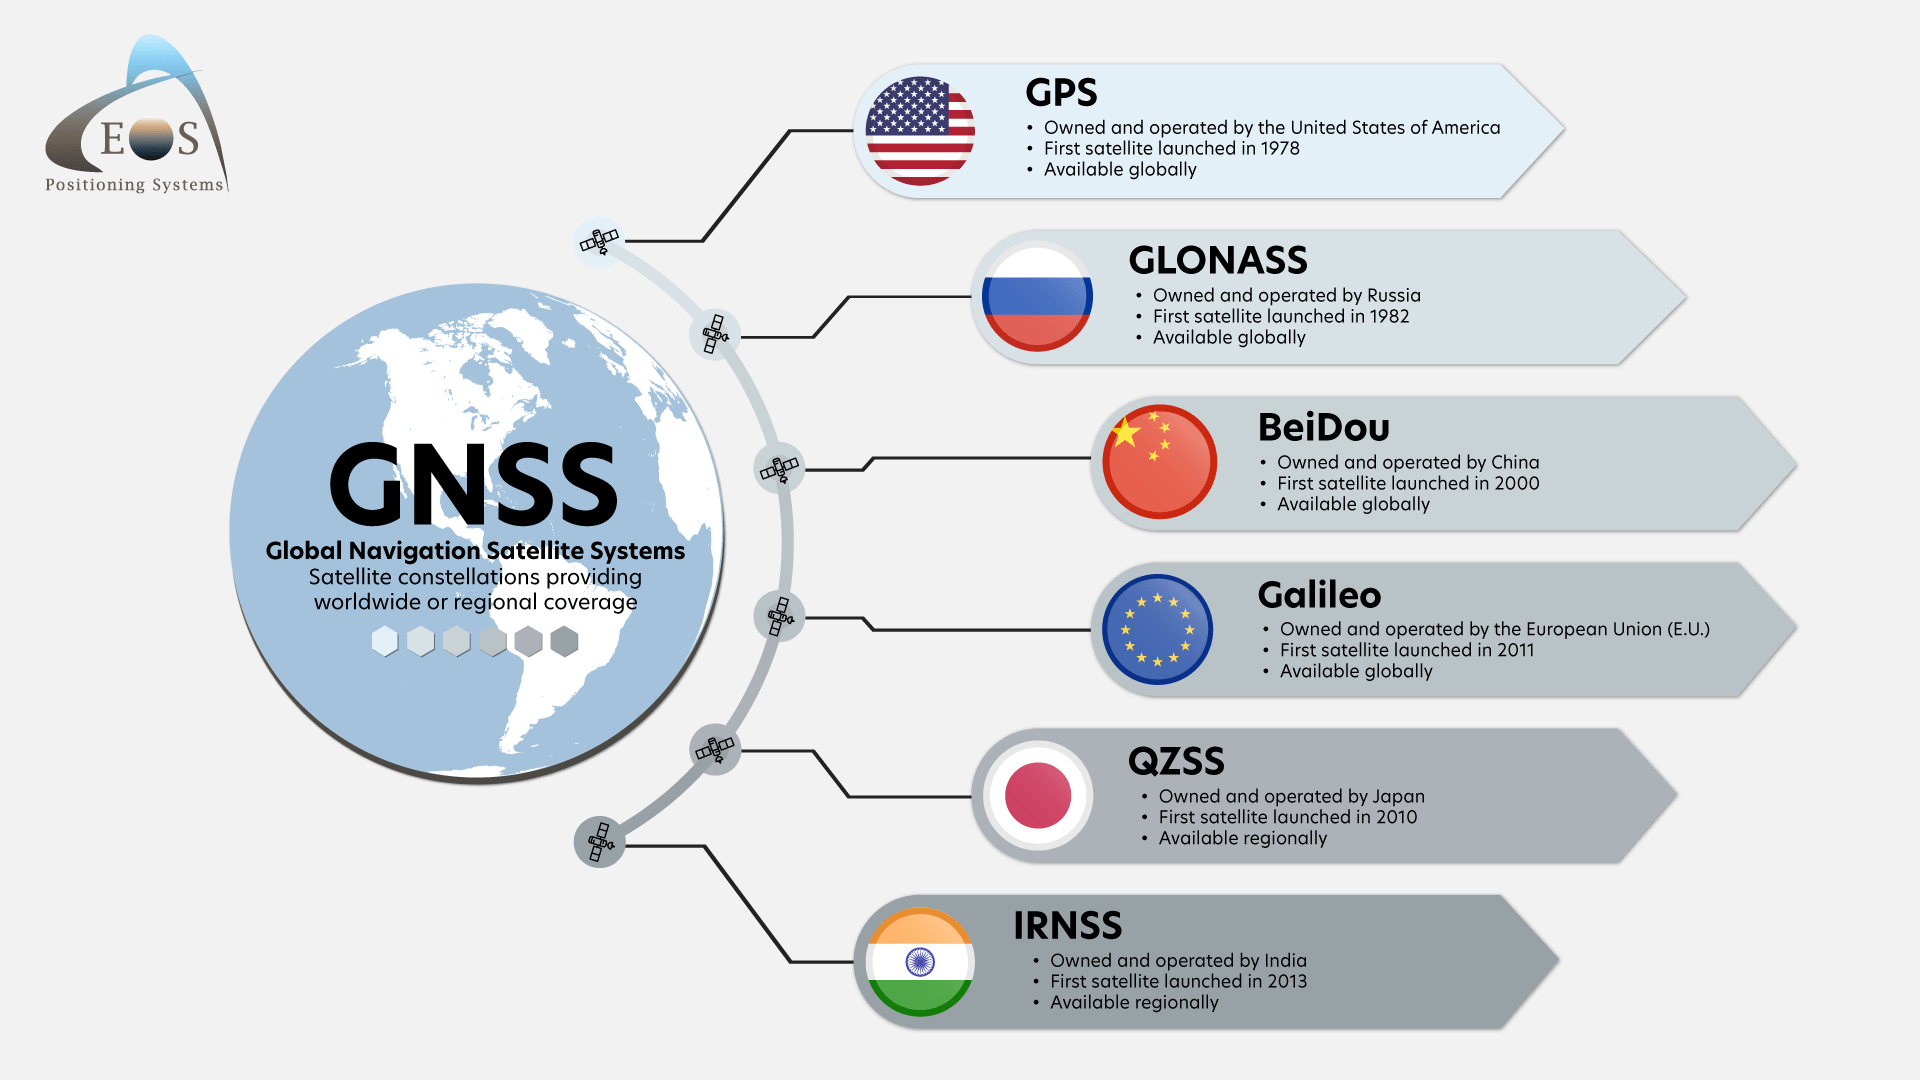
\includegraphics[width = 0.5\textwidth]{images/GNSS-Infographic-1.png}
    \caption{GNSS}
    \label{fig:enter-label}
\end{figure}

\begin{figure}
    \centering
    \includegraphics[width = 0.5\textwidth]{images/Apollo_IMU_at_Draper_Hack_the_Moon_exhibit.agr.jpg}
    \caption{IMU Sensor}
    \label{fig:enter-label}
\end{figure}

\end{columns}





\end{frame}

%------------------------------------------------

\subsection{GPS Attacks}
\begin{frame}{GPS Attacks}


\begin{columns}

\column{.5\textwidth} % Left column and width
Due to the unencrypted nature of civilian GPS signals, the GPS is vulnerable to attacks.

\begin{block}{GPS Jamming}
    Broadcasting radio signals on the same frequency as GPS satellites  to overpower or interfere with the relatively weak GPS signals received by a GPS receiver.
\end{block}

\begin{block}{GPS Spoofing (Our Focus)}
    Transmitting fake GPS signals that are structured to mimic legitimate GPS signals.
\end{block}

\column{.5\textwidth} % Right column and width

\begin{figure}
    \centering
    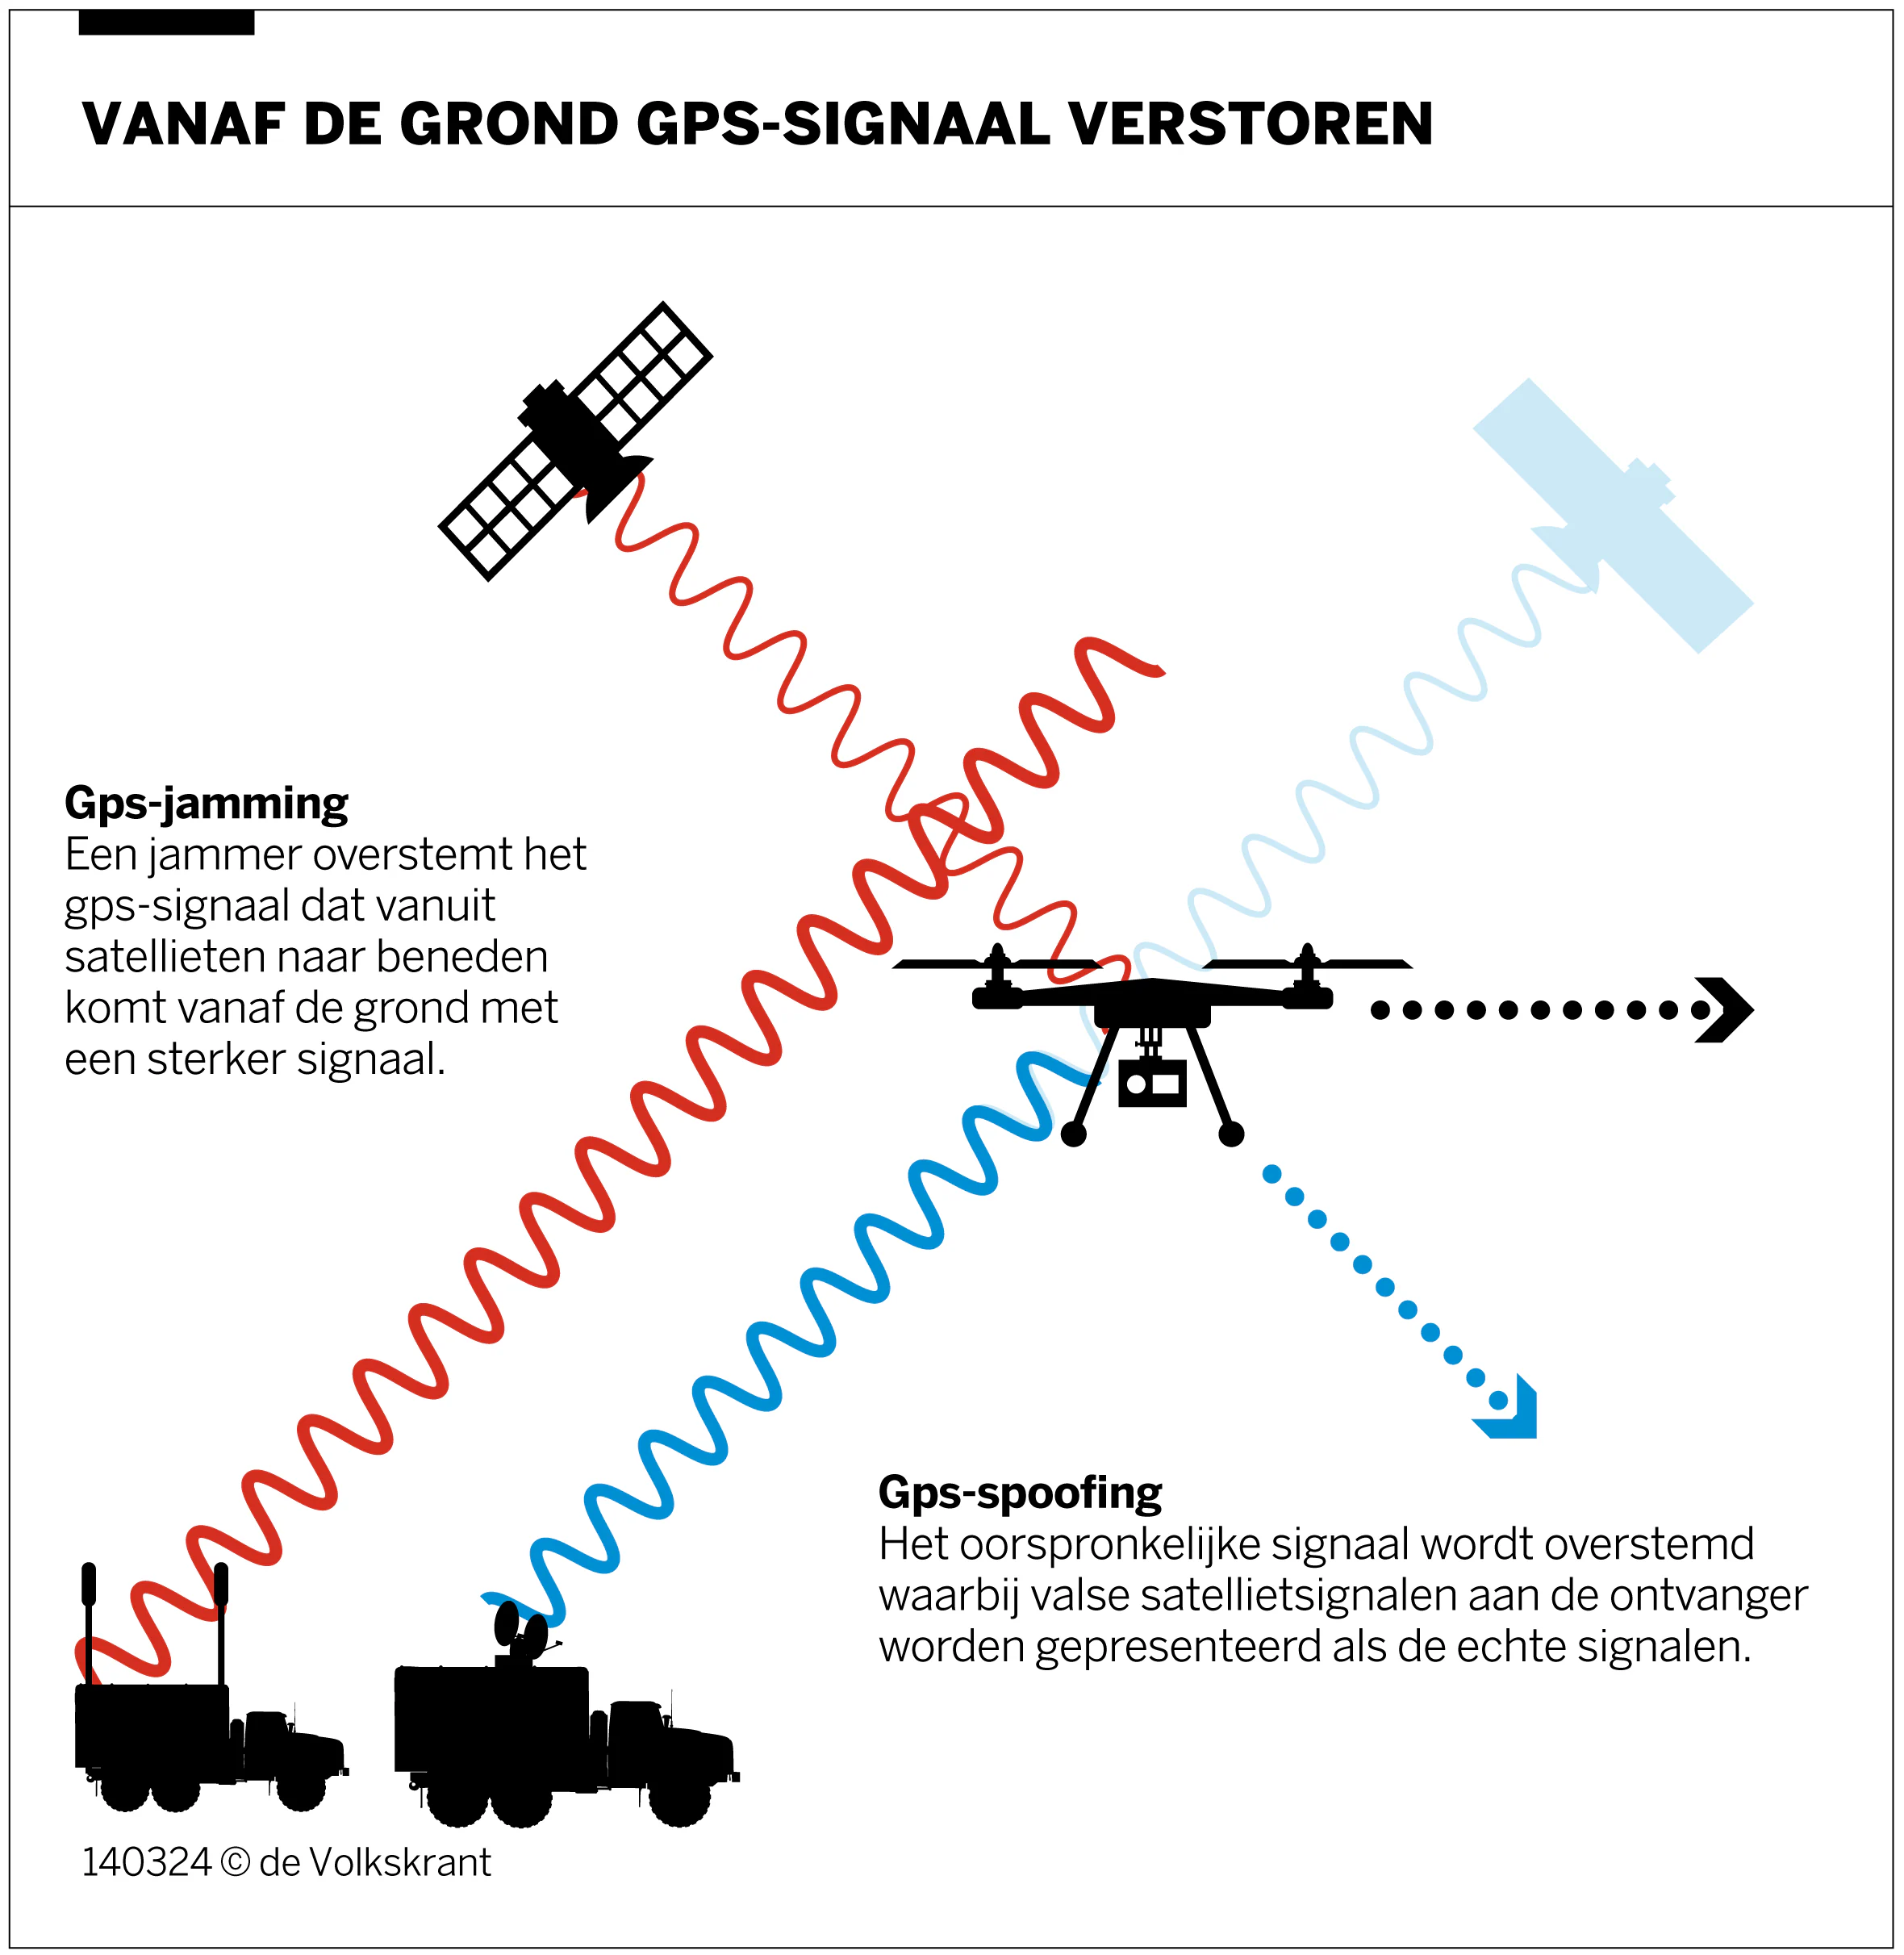
\includegraphics[width = 0.7\textwidth]{images/jamming.png}
    \caption{GPS Jamming and Spoofing}
    \label{fig:enter-label}
\end{figure}

\end{columns}






    
\end{frame}

%------------------------------------------------


% \begin{frame}
% \frametitle{Theorem}
% \begin{theorem}[Mass--energy equivalence]
% $E = mc^2$
% \end{theorem}
% \end{frame}

%------------------------------------------------

% \begin{frame}[fragile] % Need to use the fragile option when verbatim is used in the slide
% \frametitle{Verbatim}
% \begin{example}[Theorem Slide Code]
% \begin{verbatim}
% \begin{frame}
% \frametitle{Theorem}
% \begin{theorem}[Mass--energy equivalence]
% $E = mc^2$
% \end{theorem}
% \end{frame}\end{verbatim}
% \end{example}
% \end{frame}

%------------------------------------------------
\subsection{Taxonomy of GPS Spoofing Detection Methods}
\begin{frame}
\frametitle{Taxonomy of GPS Spoofing Detection Methods \footnote{Meng, L., Yang, L., Yang, W., \& Zhang, L. (2022). A survey of GNSS spoofing and anti-spoofing technology. Remote Sensing, 14(19), 4826.}}

\begin{columns}
    \begin{column}{0.5\textwidth}
        \begin{block}{ Signal processing based methods}
            Detect anomalous jumps in Signal specifications.
        \end{block}

        {\small
        \begin{itemize}
            \item  (Oligeri et al., 2019) uses cellular data to estimate UAV locations
            \item (Elena et al., 2022) proposed a method to normalize UAV signals.
        \end{itemize}
        }

    
        
    \begin{block}{ Encryption based methods}
            Utilize encryption to create unpredictable signal.
        \end{block}

        


    \end{column}
        
    \begin{column}{0.5\textwidth}
       \begin{block}{ Drift based methods}
            Detect anomalous changes on receiver's position or on clock.
        \end{block}

        {\small
        \begin{itemize}
            \item (Truong et al., 2023) utilize clock bias to detect abnormal signals.
            \item  \textbf{\textcolor{blue}{Inertial Measurement Unit} } Constraining drone's location based on velocity and acceleration.
            \item (Ian and Ryan, 2020) used two statistical methods to model the signal.
            \item (Gabriele et al., 2019) used cell sites to estimate the drone's position to detect.
            \item (Wang et al., 2020) leverages LSTM model to simulate a predicted path to compare the signals received against the predicted path. 
        \end{itemize} 
        }
        
        
        
    \end{column}
\end{columns}



\end{frame}

% ---part 2 taxonomy 
\begin{frame}
\frametitle{Taxonomy of GPS Spoofing Detection Methods \footnote{Meng, L., Yang, L., Yang, W., & Zhang, L. (2022). A survey of GNSS spoofing and anti-spoofing technology. Remote Sensing, 14(19), 4826.}}

\begin{columns}
    \begin{column}{0.5\textwidth}
         \begin{block}{ Signal/Geographical Location based methods}
            Monitor the direction of arrival of the signal by considering the received beat carrier phase.
        \end{block}
    \end{column}
        
    \begin{column}{0.5\textwidth}
        \begin{block}{ Complementary strategy of multiple detection methods}
            Mixed detection method combining multiple anti-spoofing strategies rather than a single method.
        \end{block}
        {\small
        \begin{itemize}
            \item (Chafiq and Farid, 2024) used Bayesian methods of multiple varieties. 
            \item  (Yalun et al., 2024) physically simulated the drones and usd Kalman filtering to detect attacks.
            \item (Michieletto et al., 2022) proposed a 3-step mixed modelings, together with different sensory data, to detect attacks on UAV formations and decide corresponding navigation model.
        \end{itemize} 
        }
    \end{column}
\end{columns}

\end{frame}


%------------------------------------------------

\section{Methodology}

%------------------------------------------------
\subsection{Selection of Methods}
\begin{frame}{Selection of Methods}


\begin{columns}
    \begin{column}{0.5 \linewidth}
        \textcolor{blue}{Dataset Coverage}
        \begin{itemize}
            \item Able to be conducted on a common, all-inclusive dataset.
            \item Existing datasets do not satisfy the requirements of different complex methods.
            \item Limited course timespan.
        \end{itemize}
        
        \textcolor{blue}{Reproducibility}
        \begin{itemize}
            \item Better with disclosed code examples.
            \item No transcendal mathematical modeling techniques that we are not able to taclke in the duration of the course.
        \end{itemize}
    \end{column}
    

    \begin{column}{0.5 \linewidth}
        \textbf{Choices:}

        \begin{block}{GSM (base model)}
            GSM-Based Approach (Oligeri et al. 2019).
        \end{block}

        \begin{block}{Machine Learning (Apply the model to GSM dataset)}
            Novelty-Based Approach: PCA + One-Class Classifiers (Whelan et al. 2020).
        \end{block}

        \begin{block}{Cumulation of Errors (Apply the model to GSM dataset)}
            Model-based Method (Garrett \& Gerdes, 2020).
        \end{block}
    \end{column}
\end{columns}



\end{frame}



%------------------------------------------------
\subsection{Problem Formulation}
\begin{frame}{Problem Formulation}
\begin{block}{Notations and Symbols}
    \textbf{\textcolor{blue}{$P_{GPS}$}} The received GPS location \\
    \textbf{\textcolor{blue}{$P_est$}} The estimated location by GSM signal \\
    
    \textbf{\textcolor{blue}{$x_i$}} The received signal strength by $i_th$ base station \\
    \textbf{\textcolor{blue}{$t$}} The time(ms) on each data point \\
    \textbf{\textcolor{blue}{$err$}} The distance between $p_{GPS}$ and $P_{est}$\\
    \textbf{\textcolor{blue}{$th$}} The threshold for $err$\\
    \textbf{\textcolor{blue}{$\hat{t}$}} The duration threshold \\
    \textbf{\textcolor{blue}{$v_t$}} The drone velocity at time $t$ \\
    \textbf{\textcolor{blue}{$a_t$}} The drone accelerate at time $t$ \\
     \textbf{\textcolor{blue}{GSM signal attack detection}: $1\{t_j-t_i>\hat{t}|\bigwedge_{x=i}^{j} err_x>th\}$}\\
     % \textbf{\textcolor{blue}{LSTM attack detection}: $p_{i+1}=LSTM(p_i,v_i,a_i)$}
    
\end{block}
% \begin{block}{Detection of attack by single data points}
%     PCA + One-Class Classifier, LSTM
% \end{block}
% \begin{block}{Detection of attack by sequence of anomalies}
%     GSM location estimation
% \end{block}

\end{frame}




% ----------



\section{Experiments}

\subsection{Experiment Settings}

\begin{frame}{"Drive Me Not" Dataset}
    \begin{columns}[T]
        \begin{column}{0.5\linewidth}
            {\small \textbf{Selected Dataset}}
               {\tiny Oligeri, G., Sciancalepore, S., Ibrahim, O. A., \& Di Pietro, R. (2019, May). Drive me not: GPS spoofing detection via cellular network: (architectures, models, and experiments). In Proceedings of the 12th Conference on Security and Privacy in Wireless and Mobile Networks (pp. 12-22).}
                
            \vspace{0.5cm}

            \
            \textbf{Scenario and Attacker Behavior}
            
            \begin{itemize}
                \item \textbf{Fixed Route}
                \begin{itemize}
                    \item Common for UAVs carrying out patrol missions and transporting missions
                \end{itemize}
                \item \textbf{Regularity}
                \begin{itemize}
                    \item The flight path and parameters in a normal flight condition have certain regularity / learnable patterns.
                \end{itemize}
                \item \textbf{Attacker}
                \begin{itemize}
                    \item \textbf{Attacker Knowledge} The attacker can know the starting point and return point of the target UAV, and can track the current speed, position and other information of the UAV. 
                    \item \textbf{Objective of the Attacker} spoof the UAV to the route set by the attacker.
                \end{itemize}
                % \item The attacker launches an attack from the ground and is able to receive satellite GPS signals and transmit higher intensity signals.
               
            \end{itemize}
                
        \end{column}
        \begin{column}{0.6\linewidth}
            \begin{figure}
                \centering
                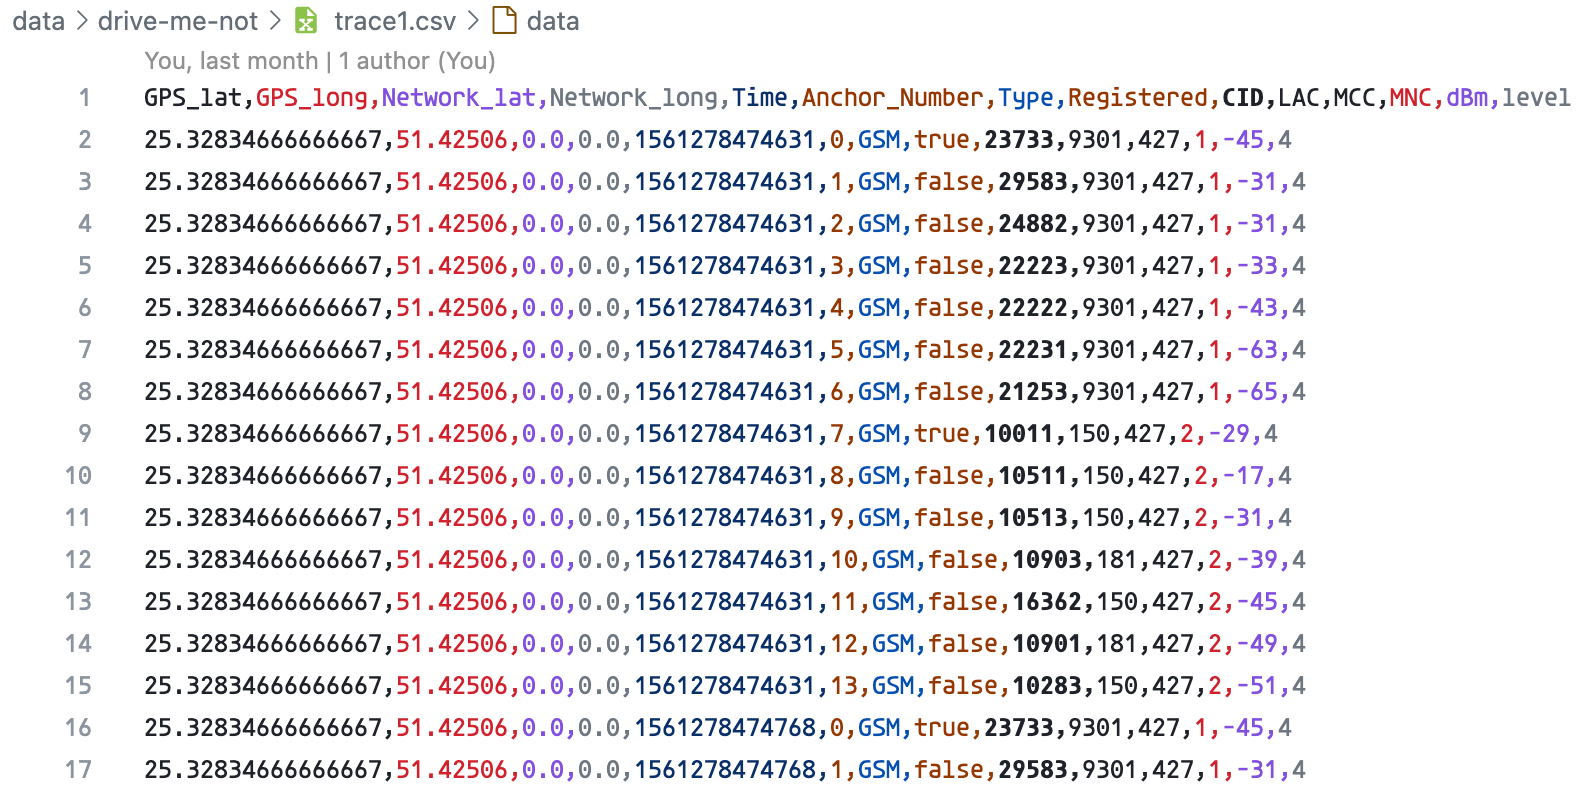
\includegraphics[width = \linewidth]{images/drive-me-not-data.png}
                \caption{Example of original trace data}
                \label{fig:enter-label}
            \end{figure}
        \end{column}
    \end{columns}
\end{frame}
% ---------
% \begin{frame}{Scenario and Attacker Behavior}
%     \begin{columns}[T]
%         \begin{column}{0.5\linewidth}
%             \begin{itemize}
%                 \item Fixed Route
%             \end{itemize}
        
%         \end{column}
        
%         \begin{column}{0.5\linewidth}
            

            
%         \end{column}
%     \end{columns}
% \end{frame}

% ---------

\begin{frame}{Generation of Datasets - Sensor Data}
    \begin{columns}[T]
        \begin{column}{0.5\linewidth}
           \textbf{Generation of IMU sensor data} 
           \begin{itemize}
               \item For (Whelan et al. 2020): Lacking 85 Sensory Data columns.  
               \item To generate velocity and acceleration data from the traces.
               \item \textcolor{blue}{Cons}: Choppy and zigzaggy data, not smooth.
               \item Differentiation? Moving Average? Outlier Handling?
           \end{itemize}

           \begin{figure}
                \centering
                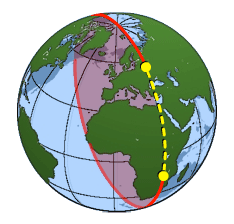
\includegraphics[width = 0.4 \linewidth]{images/haversine.png}
                \caption{\textcolor{blue}{Haversine distance} is needed for calculating distance from coordinates}
                \label{fig:enter-label}
            \end{figure}

            
        \end{column}
        
        \begin{column}{0.5\linewidth}
           \begin{figure}
               \centering
               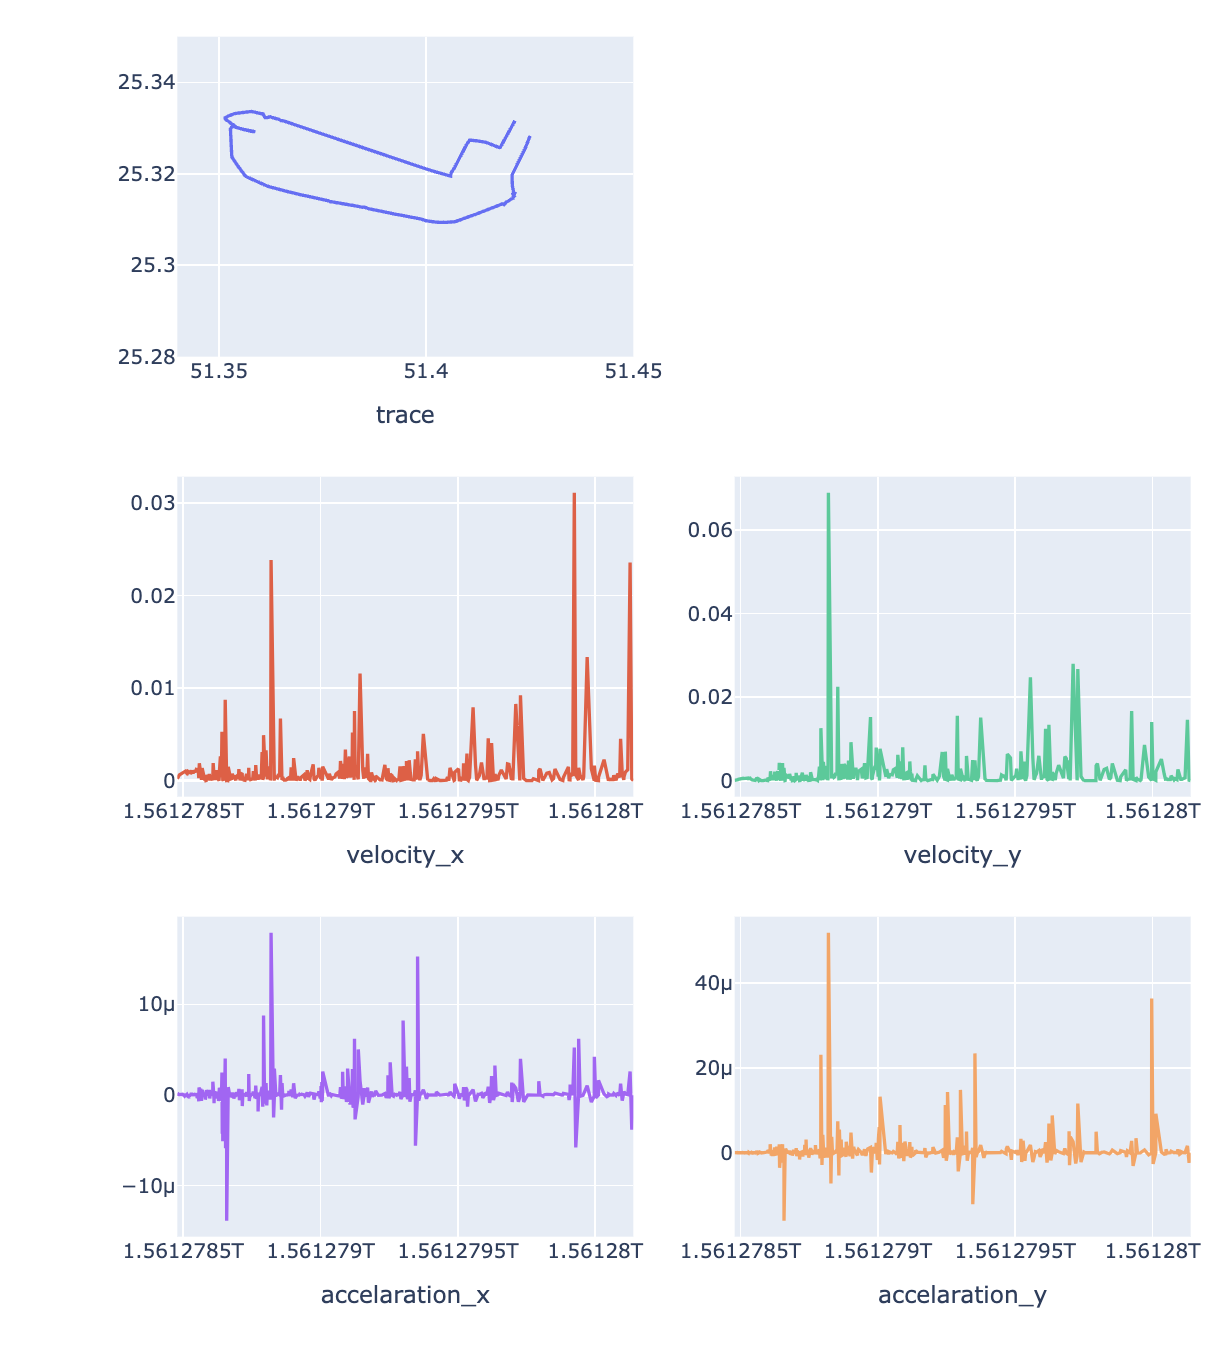
\includegraphics[width=0.7\linewidth]{images/velocity-generation.png}
               \caption{Example: Generated Velocity / Acceleration Data w.r.t the Original Trace of Trace 1}
               \label{fig:enter-label}
           \end{figure}
            
        \end{column}
    \end{columns}
\end{frame}

% \begin{frame}
%     \begin{columns}[T]
%         \begin{column}{0.5\linewidth}
           

           
            
%         \end{column}
        
%         \begin{column}{0.5\linewidth}



            
%         \end{column}
%     \end{columns}
% \end{frame}


% ---------

\begin{frame}{Generation of Datasets - Spoofed Traces}

\begin{itemize}
    \item \large{Randomly selecting a direction.}
    \item \large{Simulating the speed in Normal Distribution among every data point.}
    \item \large{Spoofing starting from the middle of the benign trace.}
\end{itemize}

\begin{figure}
    \centering
    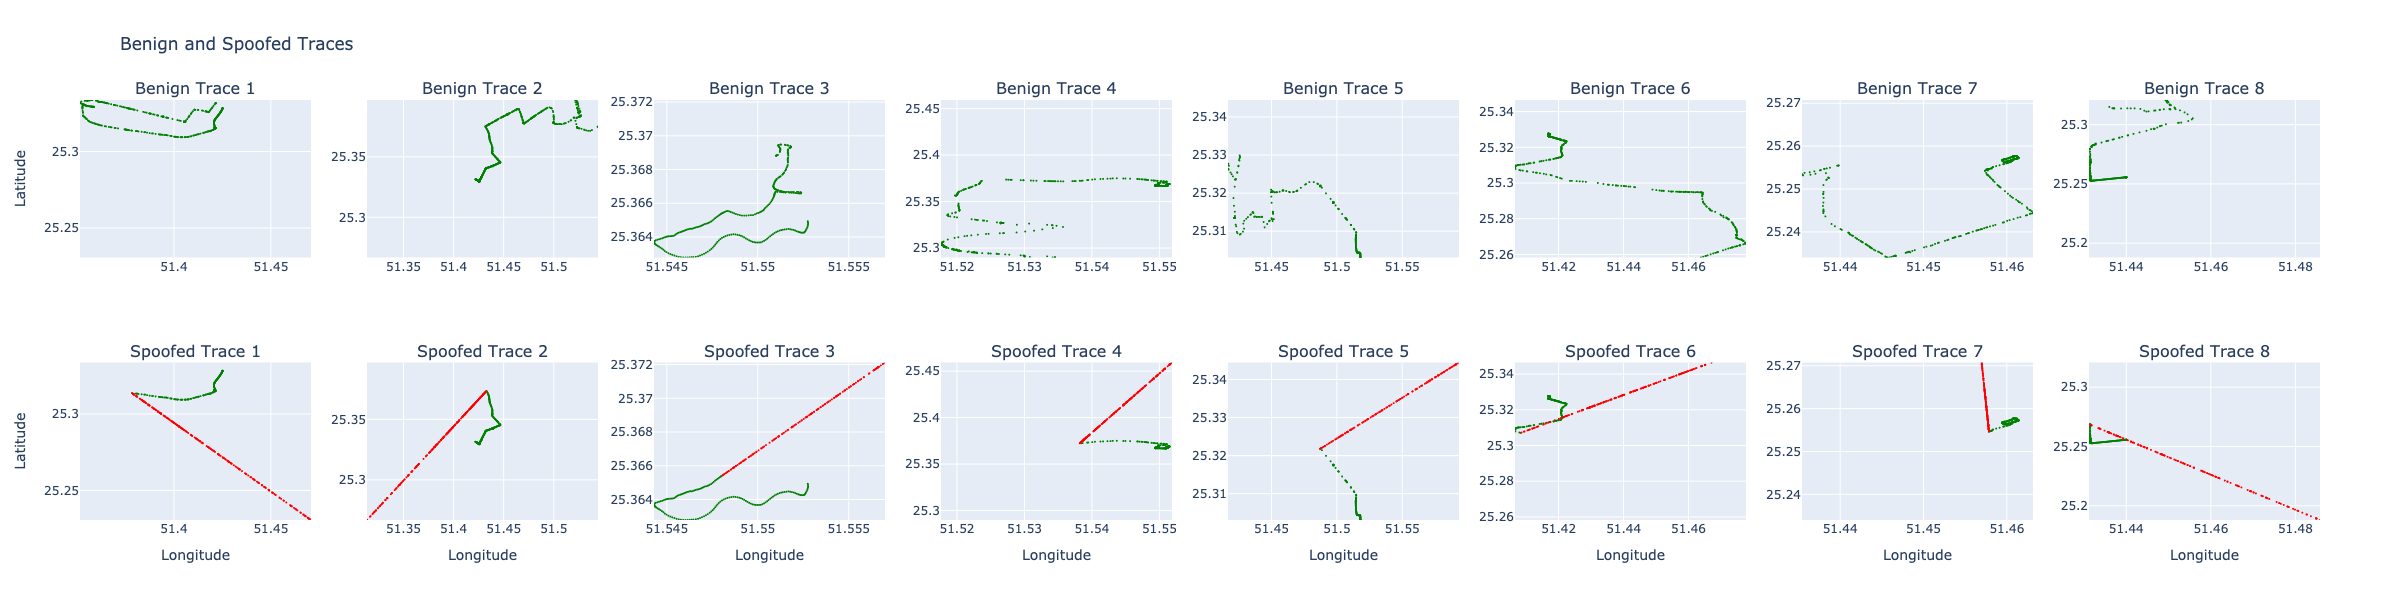
\includegraphics[width=\linewidth]{images/traces.png}
    \caption{Spoofed Traces Used }
    \label{fig:enter-label}
\end{figure}

\end{frame}










%------------------------------------------------
\subsection{GSM-Based Approach (Oligeri et al. 2019)}
\begin{frame}{GSM (Oligeri et al. 2019)}
\begin{columns}[T]
    \begin{column}{0.5\linewidth}
    
    \begin{block}{Cellular Network Position Estimation}
                GSM + UMTS
    \end{block}
    
    \begin{block}{Received Signal Strength Modelling}
                Using Exponential Distribution to calculate the weight of base stations.
    \end{block}        
    
    \end{column}

    \begin{column}{0.5\linewidth}

\begin{figure}
            \centering
            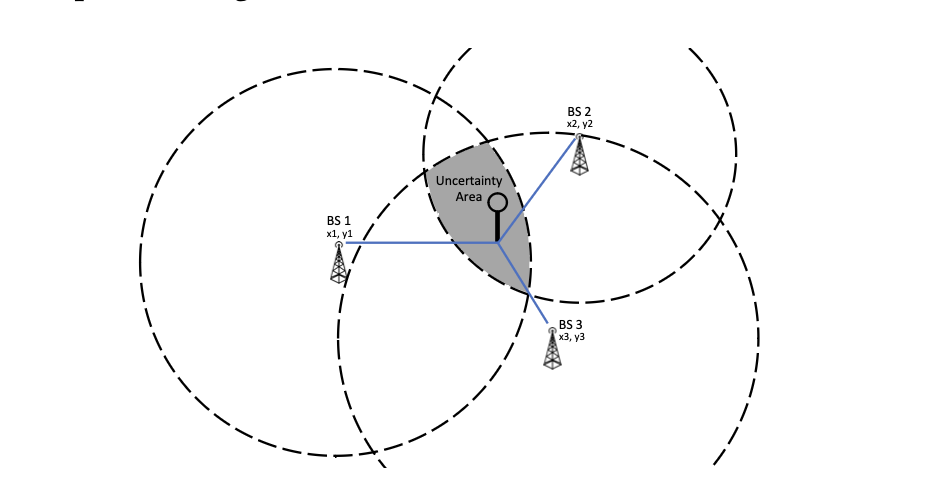
\includegraphics[width = 0.5 \textwidth]{images/basestation.png}
            \caption{Position relation between base station and drone}
            \label{fig:bs}
        \end{figure}

    
    \end{column}
\end{columns}
\begin{figure}
            \centering
            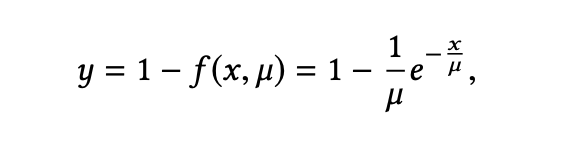
\includegraphics[width = 0.4 \textwidth]{images/expo.png}
            % \caption{The weight of base station with RSS}
            \label{fig:expo}
        \end{figure}
\begin{equation}
    \large w_i=\frac{y_i}{\sum_{i=1}^{N}y_i}
\end{equation}
\end{frame}



\begin{frame}{Model Parameters}
\begin{block}{Model Parameters}
\begin{itemize}
    \item \textbf{$\mu$ in Exponential Distribution:} Minimizing the distance between GPS location and Estimated GSM location. \vspace{1em}
    \item \textbf{Anomaly threshold:} The difference between 2 locations beyond the threshold as anomaly. \vspace{1em}
    \item \textbf{Anomaly sequence duration threshold:} The anomaly sequence duration beyond the threshold as attack.
    \vspace{1em}
\end{itemize}

    
\end{block}

                

\end{frame}


\begin{frame}{Effectiveness}


\begin{columns}[T]
    \begin{column}{0.5\linewidth}
    
      \begin{itemize}
               
                \item A lot of base stations around every location.
            \end{itemize}

        \begin{figure}
            \centering
            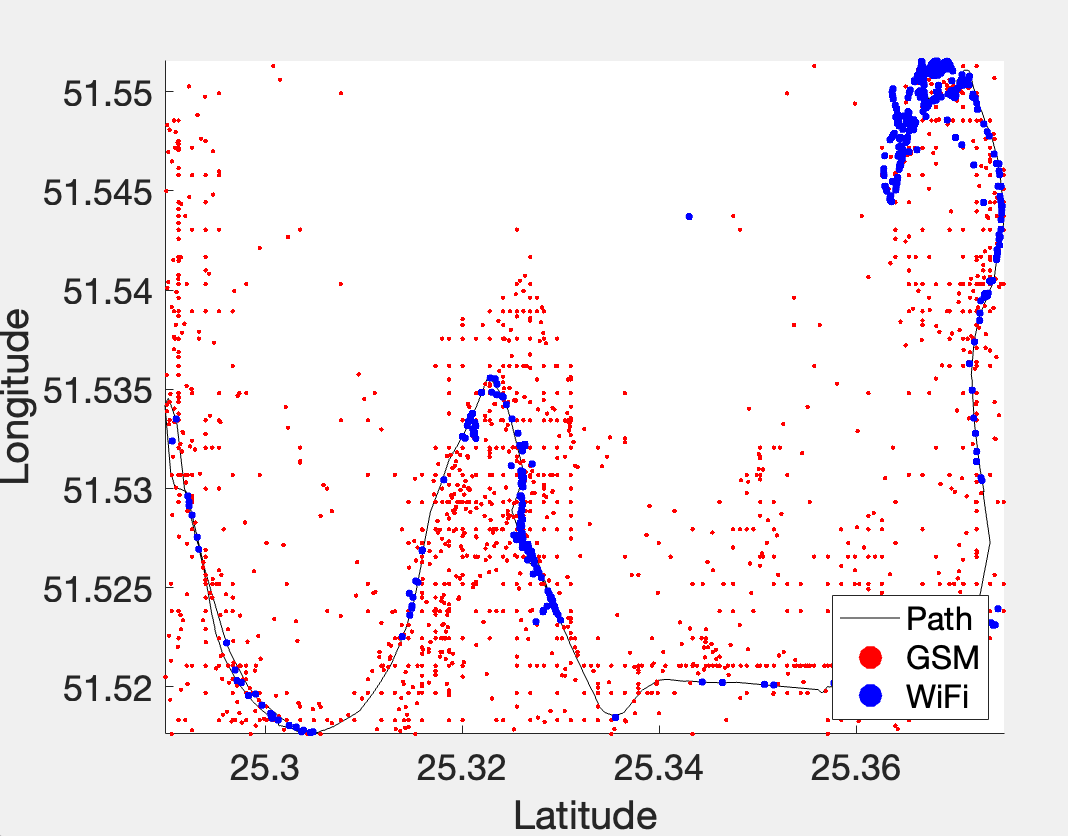
\includegraphics[width = 0.7 \textwidth]{images/path_gsm.png}
            \caption{One UAV trace with base station location}
            \label{fig:path_gsm}
        \end{figure}
    \end{column}

    \begin{column}{0.5\linewidth}
\begin{itemize}
                \item UAV receives 11-15 Base station signals in most of positions.
               
            \end{itemize}


    \begin{figure}
            \centering
            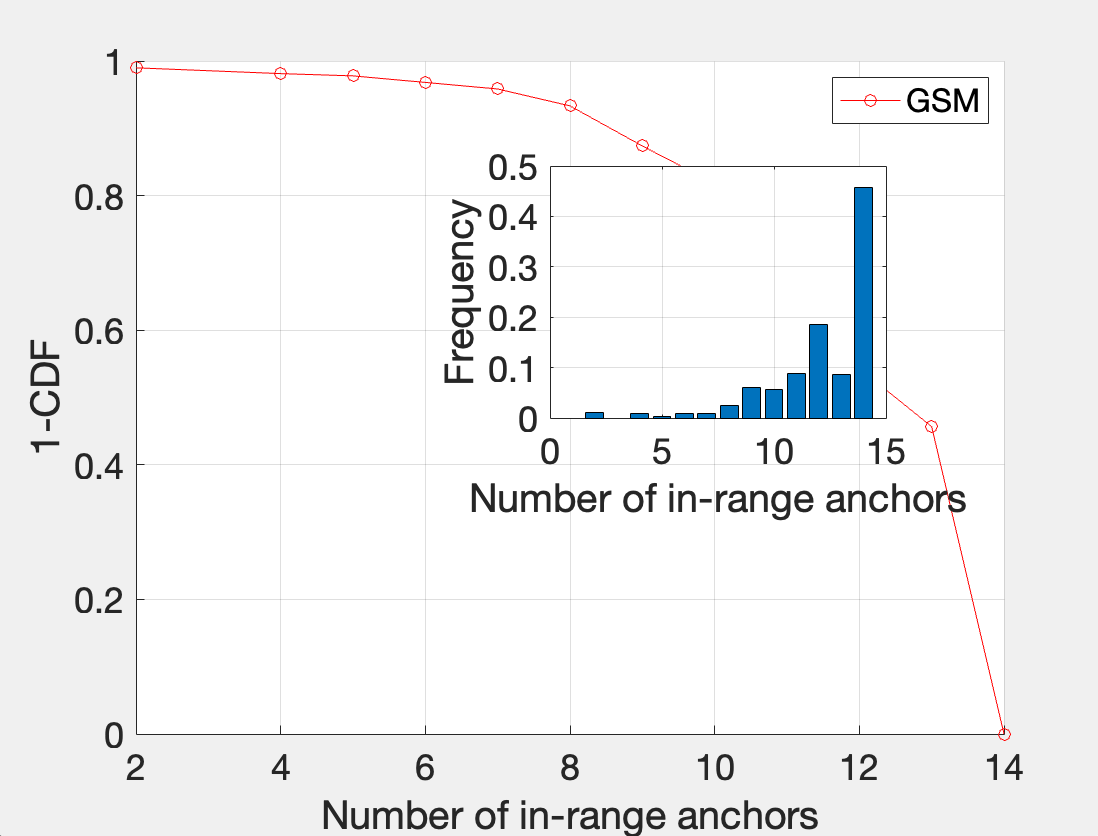
\includegraphics[width = 0.7 \textwidth]{images/num_bs.png}
            \caption{The distribution of received base station signals}
            \label{fig:num_bs}
        \end{figure}
    \end{column}
\end{columns}



\end{frame}


\subsection{GSM-Based Approach: Experiment (Oligeri et al. 2019)}




\begin{frame}{Threshold Estimation}

    \begin{columns}
        \begin{column}{0.6\linewidth}
        \begin{block}{Datasets}
            \begin{itemize}
                \item 8 traces collected from Doha, Qatar, driving more than 150km for about 10 hours (Gabriele et al. 2019).
                \item Trace4 as an example:\\
                Y\_est: position estimated by mobile cellular network.\\
                X\_GPS: position received by the GPS (real signal and our generated spoof signal).
            \end{itemize}
        \end{block}
            % \begin{block}{Distance}The threshold of distance between the received GPS location and the estimated location by GSM signal
            
            % \end{block}
            
            % \begin{block}{Duration}
            % The Duration of anomalies beyond threshold.
            % \end{block}
        \begin{figure}
            \centering
            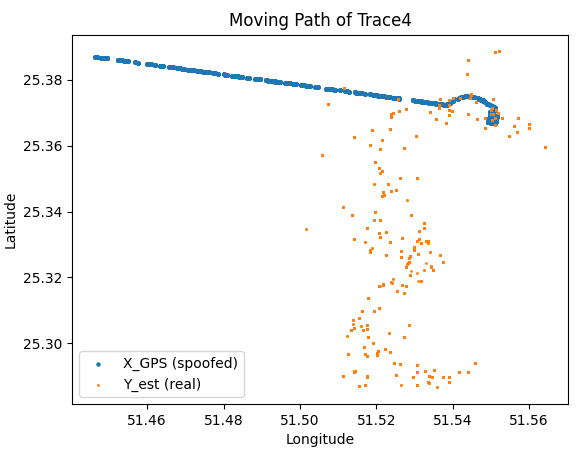
\includegraphics[width = 0.6\textwidth]{images/trace4.png}
            \label{fig:enter-label}
        \end{figure} 
        \end{column}
        
        \begin{column}{0.4\linewidth}
            \begin{figure}
                \centering
                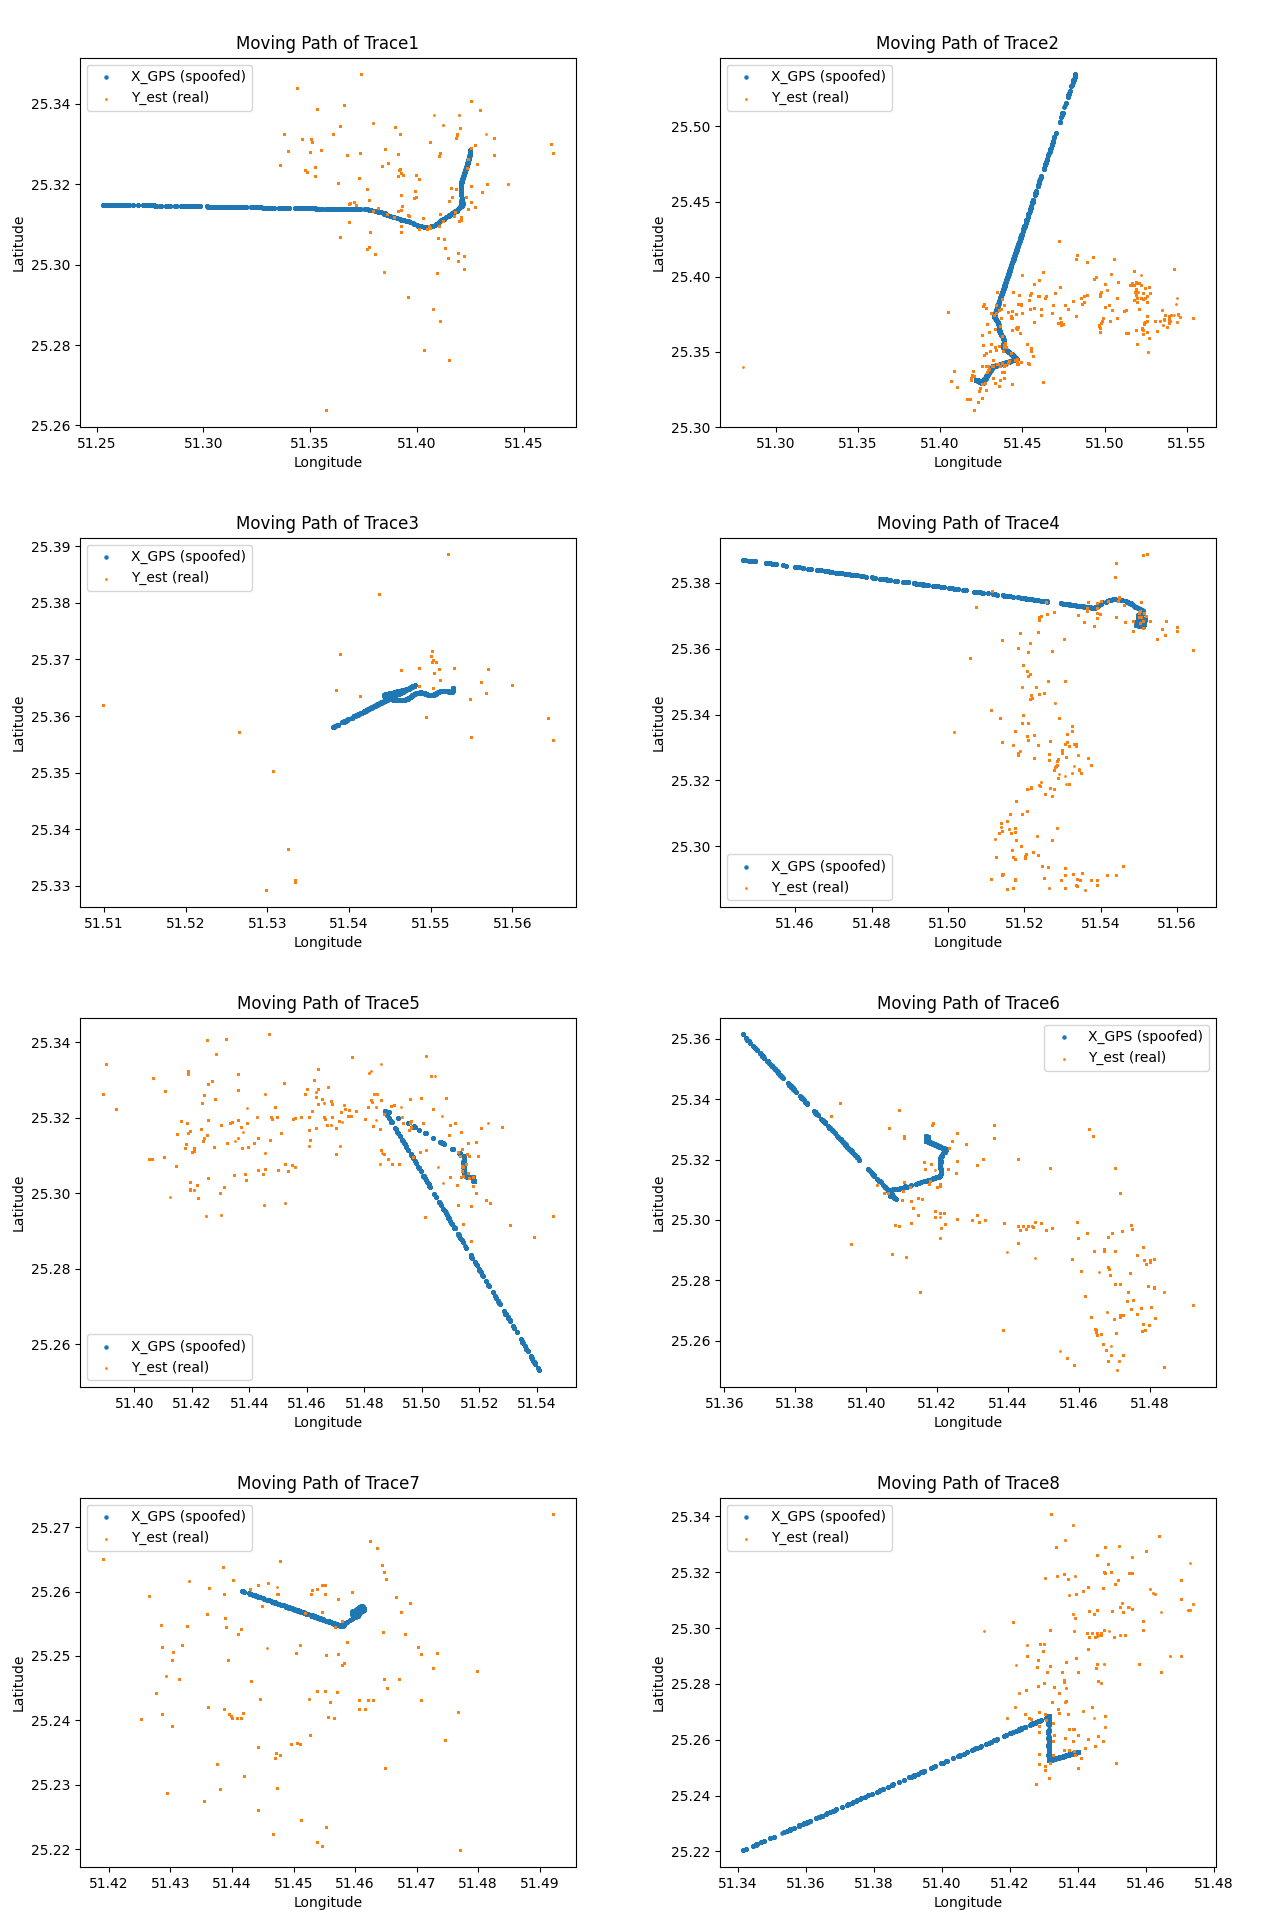
\includegraphics[width = 0.5\textwidth]{images/Garrett_moving_path.png}
                \label{fig:enter-label}
            \end{figure}
           \begin{itemize}
               \item \textbf{Train and Test dataset} \\
                Train set: Trace 5-8 \\
                Test set: Trace 1-4
            \end{itemize}
            \begin{itemize}
                \item \textbf{Training policy} \\
                Minimizing the duration and distance before spoofed trace being detected
             \end{itemize}
    
           
       \end{column}
    \end{columns}
    
    
\end{frame}


\begin{frame}{Experiment Results}

\begin{itemize}
    \item \textbf{\large{Determine the ideal threshold using data quantiles.}}
 
\end{itemize}
\begin{figure}[h]
  \centering
  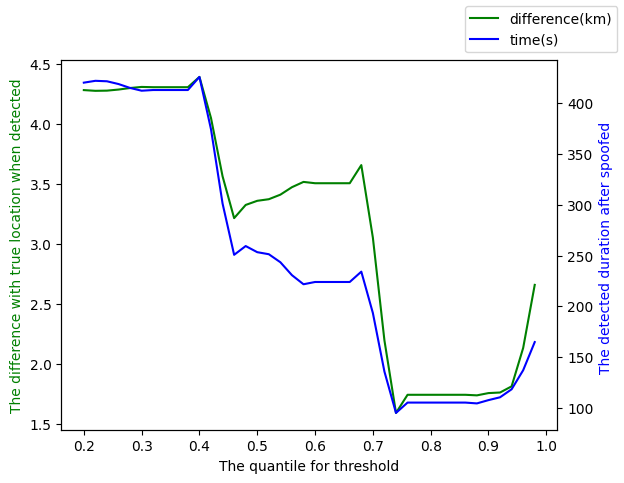
\includegraphics[width=0.55\linewidth]{images/quantile.png}
  \caption{Detection duration and distance relative to the quantile of the training dataset}
  \Description{}
  \label{quantile}
\end{figure}

\end{frame}


\begin{frame}{Experiment Results}
\begin{block}{Duration of anomaly sequence}
Guarantee 0 false positive rate in training dataset and minimalize the detection duration and distance.
\end{block}
\begin{table}[h]
    \centering
    \begin{tabular}{lccc}
        \toprule
        \textbf{Datasets} & \textbf{False Positive} & \textbf{Duration} & \textbf{Distance} \\
        \midrule
        trace1  & 0.17  & 100.4 & 2.23 \\
        trace2  & 0.11  & 93.3 & 1.33 \\
        trace3  & 0   & 93.6 & 0.94 \\
        trace4  & 0.05   & 151.0 & 1.34 \\
        trace5  & 0  & 173.9 & 1.83 \\
        trace6  & 0  & 96.4 & 1.57 \\
        trace7  & 0  & 155.1 & 1.74 \\
        trace8  & 0  & 144.0 & 1.41 \\
        \bottomrule
    \end{tabular}
    \caption{Drive me not model}
    \label{tab:dmn}
\end{table}

    
\end{frame}
%------------------------------------------------



%------------------------------------------------
\subsection{Novelty-Based Approach: PCA + One-Class Classifiers (Whelan et al. 2020)}
\begin{frame}{PCA + One-Class Classifiers}


\begin{columns}[T]
    {\small
    \begin{column}{0.5\linewidth}
        
        Make use of a variety of sensor data.
    
        \begin{block}{Principle Component Analysis (PCA)}
            \begin{itemize}
                \item  Decompose to a set orthogonal components with explainability on most of the variance.
                \item  (Whelan et al. 2020) Reduce 85 features to 3 principal components.
                \item Fit PCA on the training set to  transform both the testing and training set.
            \end{itemize}
        \end{block}

        Feed the reduced components into the OCC models.
        \begin{block}{Novelty Detection with One-Class Classifiers}
            \begin{itemize}
                \item Does \textbf{not} require anomalies to pre-exist in the dataset during training.
                \item New observations outside of learned distribution are classified as \textbf{novelties}.
                \item Can be pre-trained. Requires only flight logs.
            \end{itemize}
        \end{block}
    \end{column}
    
    \begin{column}{0.5\linewidth}
        \begin{figure}
            \centering
            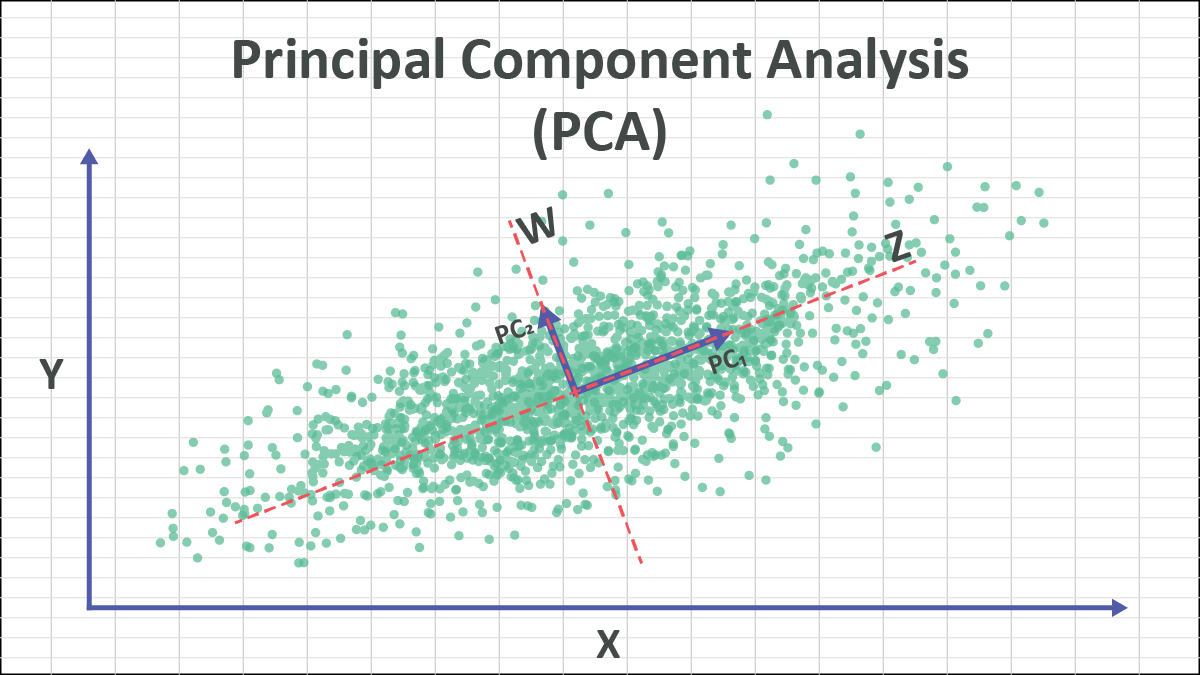
\includegraphics[width = 0.5 \textwidth]{images/principal-component-analysis-pca-featured.png}
            \caption{PCA constructs PCA components with low dimensions}
            \label{fig:pca-1}
        \end{figure}

        \begin{figure}
            \centering
            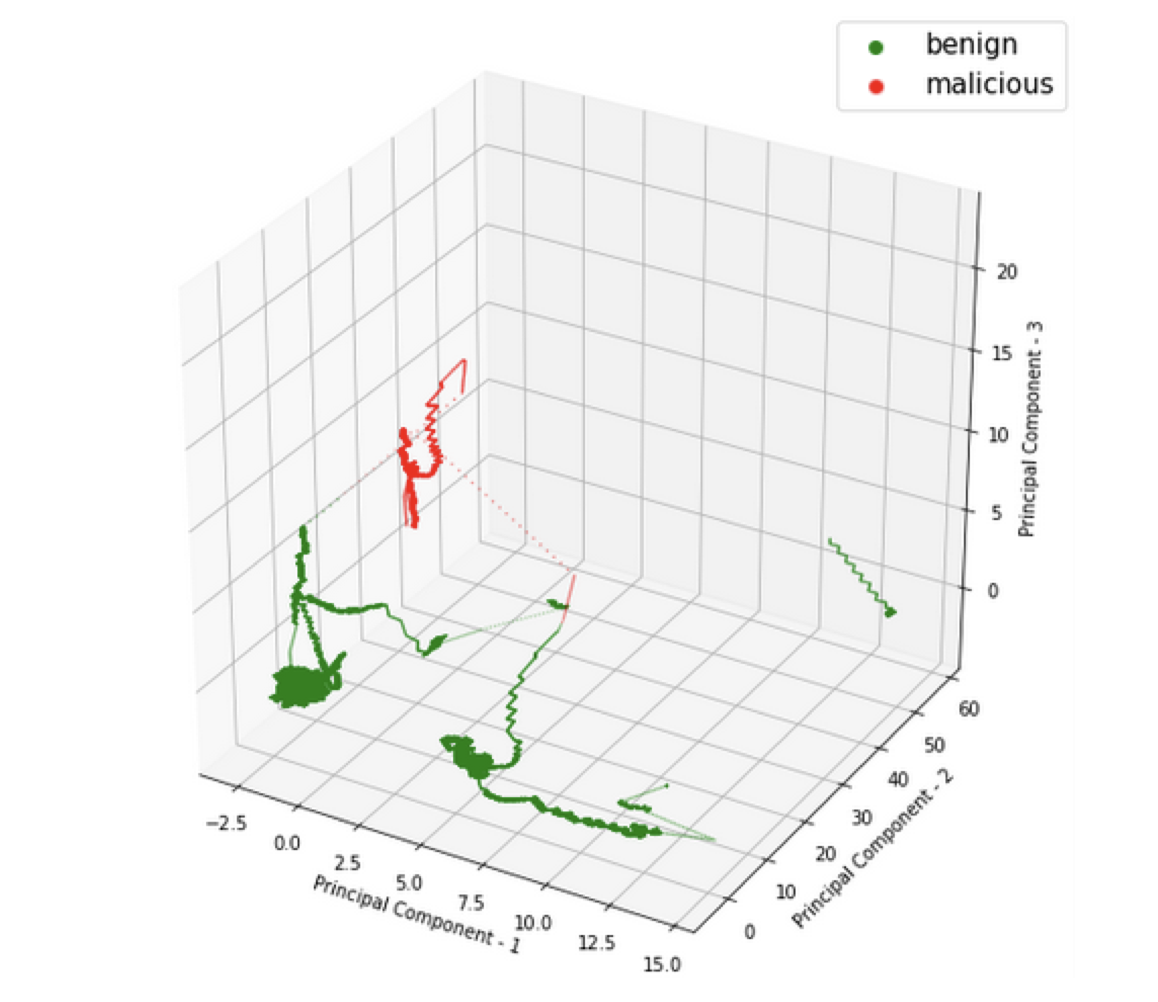
\includegraphics[width = 0.5 \textwidth]{images/whelan-pca.png}
            \caption{Reduced components in 3d space (Whelan et al., 2020)}
            \label{fig:pca-2}
        \end{figure}
    \end{column}
    }
\end{columns}

\end{frame}

%  ----

\begin{frame}{One-Class Classifiers for Novelty Detection}

\begin{columns}[T]

    \begin{column}{0.5\linewidth}

    
    
        \begin{block}{One-Class SVM (OCSVM)}
            \begin{itemize}
                \item Unsupervised anomaly detection algorithm.
                \item Extension of SVM to distinguish the majority of data points from outliers.
            \end{itemize}
            % Unsupervised anomaly detection algorithm that learns a decision boundary to distinguish the majority of data points from outliers, by finding the maximum margin hyperplane that separates the training data from the origin in a high-dimensional feature space.
        \end{block}



        \begin{block}{Local Outlier Factors (LOF)}
            \begin{itemize}
                \item Unsupervised density-based anomaly detection algorithm.
                \item Assigns an \textcolor{blue}{outlier score} to each data point based on the local density of its \textcolor{blue}{neighborhoods}.
                \item \textcolor{blue}{Outliers}: points with significantly lower density than their neighbors.
            \end{itemize}

        \end{block}
    \end{column}
    
    \begin{column}{0.5\linewidth}
        \begin{figure}
            \centering
            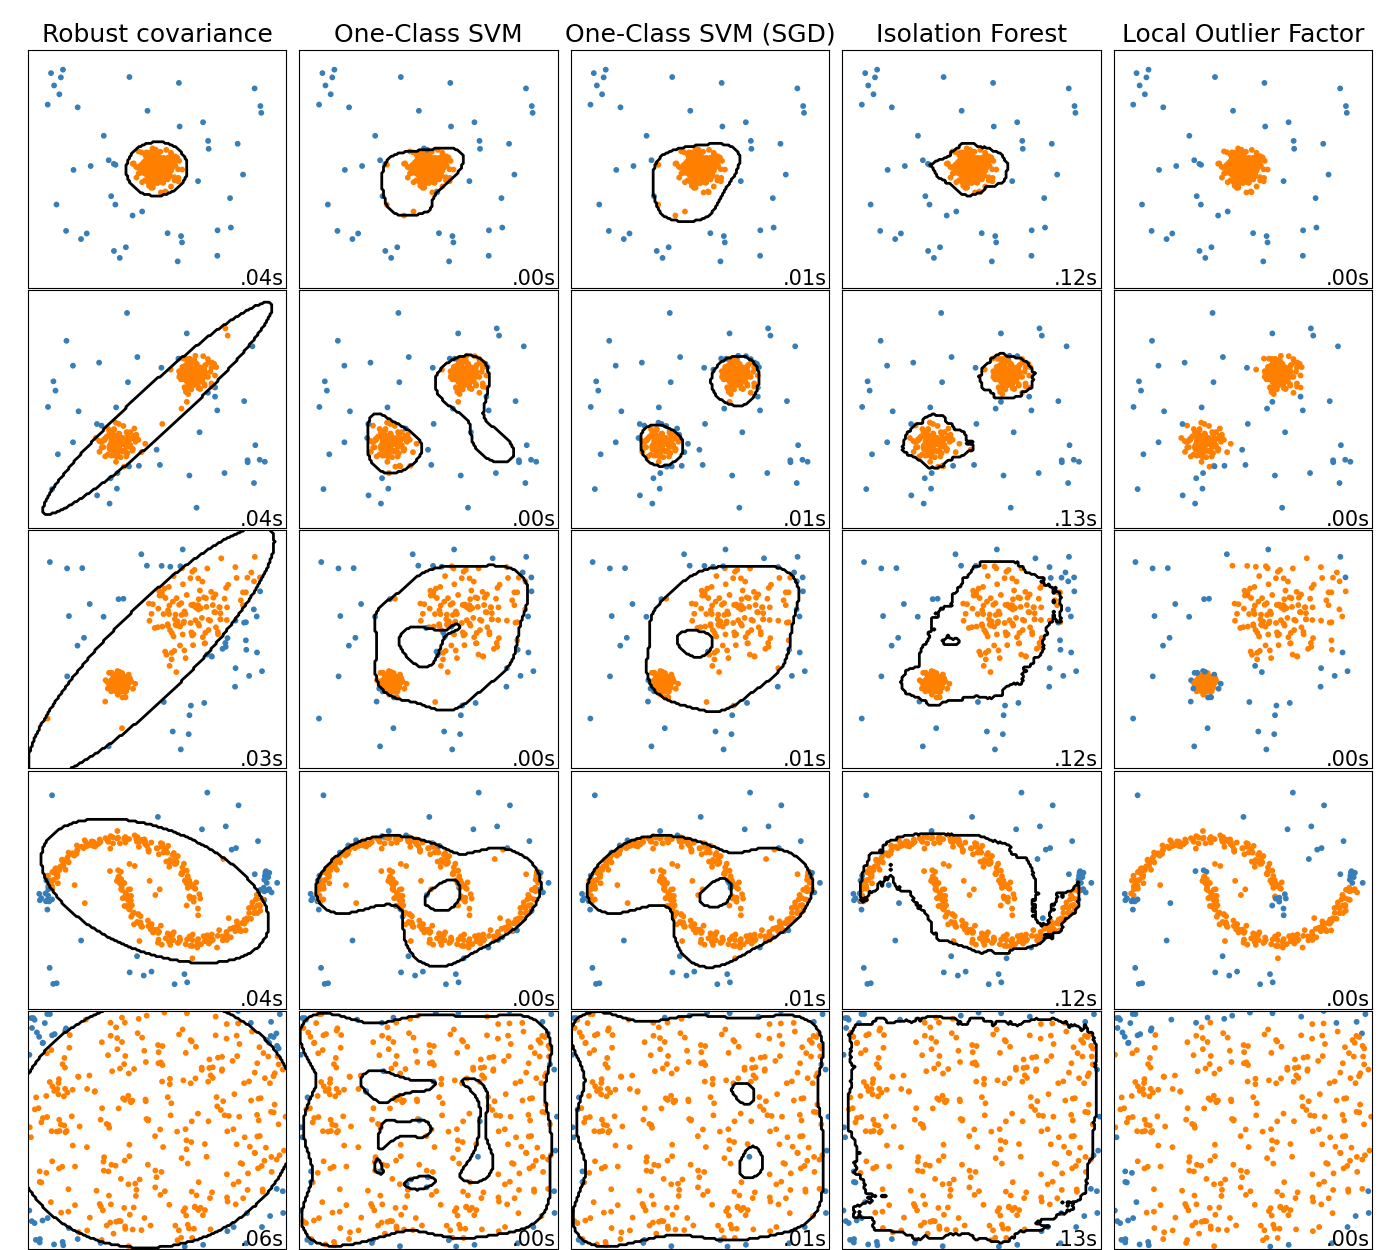
\includegraphics[width = 0.8\textwidth]{images/oc.png}
            \caption{One-Class Classifier demonstration from sklearn documentation \url{https://scikit-learn.org/stable/modules/outlier_detection.html#overview-of-outlier-detection-methods} }
            \label{fig:enter-label}
        \end{figure}
    \end{column}
\end{columns}

\end{frame}

\begin{frame}{One-Class Classifiers for Novelty Detection}


\begin{columns}[T]

    \begin{column}{0.5\linewidth}
    
        \begin{block}{Autoencoder}
            \begin{itemize}
                \item \textcolor{blue}{Hidden encoded layer}: compression-decompression reconstruction.
                \item \textcolor{blue}{Only benign data are supposed to reconstruct itself} from the model.
                \item Trained on a benign dataset with MSE loss.
                
                \item Compare the MSE difference of the reconstructed input with a Threshold \(T\)
                (how to choose the threshold is not disclosed in (whelan et al. 2020)).
            \end{itemize}
                    
        \end{block}
        
    \end{column}
    
    \begin{column}{0.5\linewidth}
        \begin{figure}
            \centering
            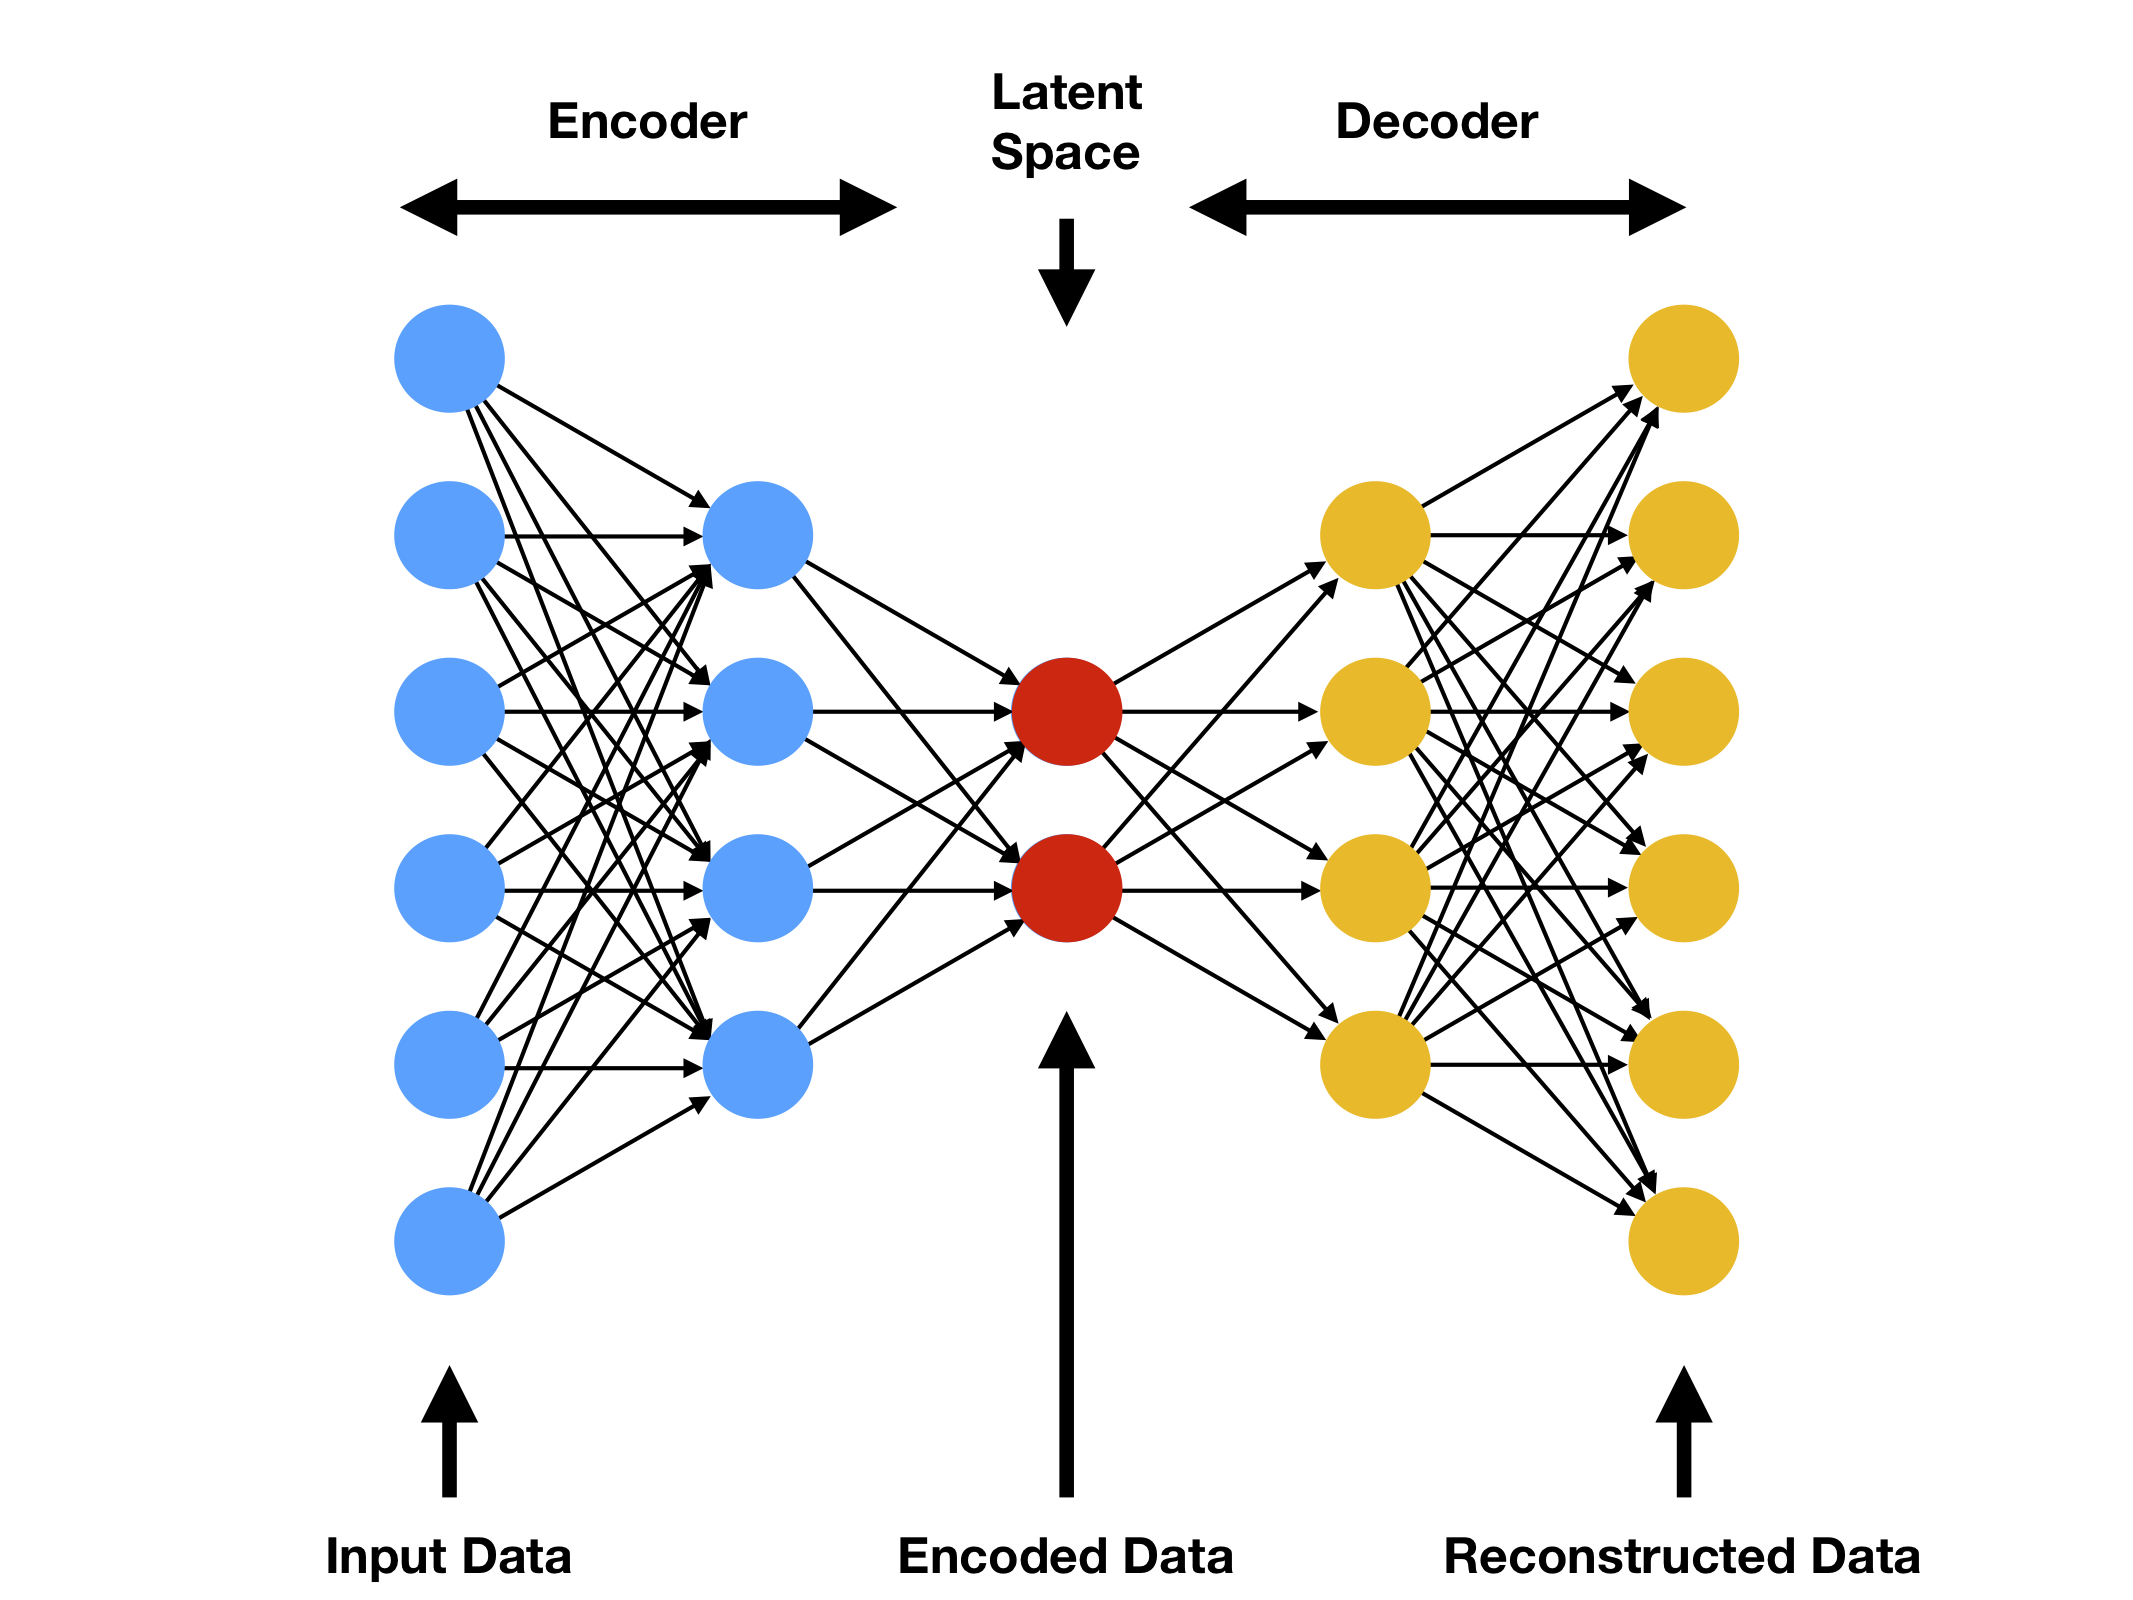
\includegraphics[width = \textwidth]{images/ae.png}
            \caption{The Autoencoder reconstructs the input data.}
            \label{fig:enter-label}
        \end{figure}
    \end{column}
\end{columns}

\end{frame}




% -------
\subsection{Novelty-Based Approach: Experiment (Whelan et al. 2020)}

\begin{frame}{Principle Component Analysis Results}

\begin{columns}

\begin{column}{0.3 \linewidth}
    \begin{itemize}
        \item Inputs: \texttt{[GPS\_lat, GPS\_lon, v\_lat, v\_lon, a\_lat, a\_lon]}
        \item Num\_Components = 3.
        \item Patterns?
    \end{itemize}
\end{column}


\begin{column}{0.7 \linewidth}
    \begin{figure}
        \centering
        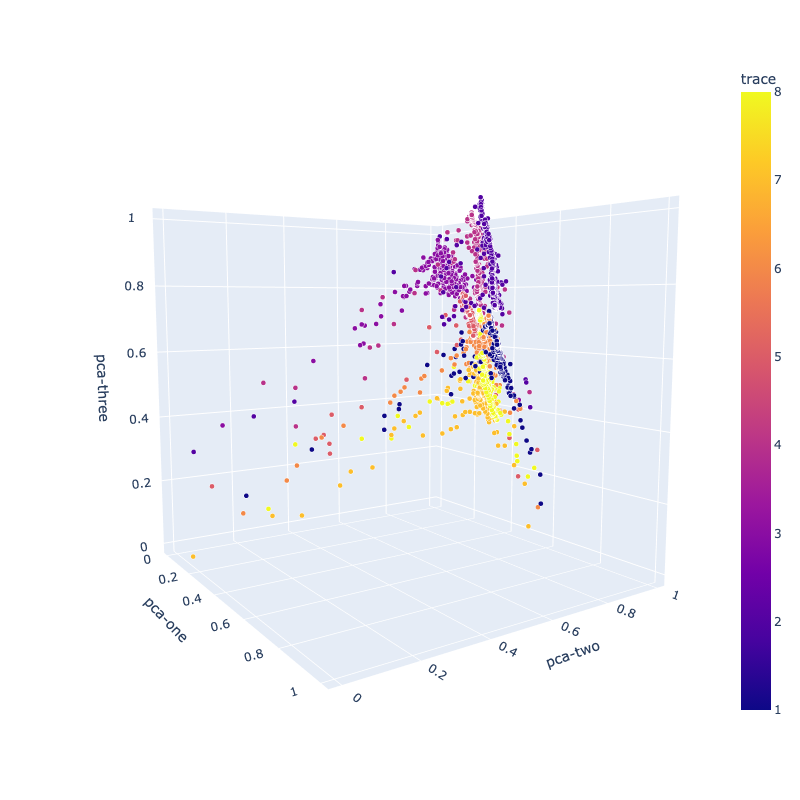
\includegraphics[width = 0.6\linewidth]{images/newplot.png}
        \caption{Visualization of PCA components}
        \label{fig:enter-label}
    \end{figure}
\end{column}

\end{columns}



\end{frame}
%-----------------------
\begin{frame}{One-Class SVM Results}
\begin{columns}

\begin{column}{0.4 \linewidth}
    \textcolor{blue}{\large{Training on traces, tested on each trace}}
    \begin{itemize}
        \item Grid search on optimal \(\nu\) and \(\gamma\) of OCSVM.
        \item Indiscriminately label all points in the test set as malicious.

    \end{itemize}
\end{column}


\begin{column}{0.7 \linewidth}
\begin{figure}
    \centering
    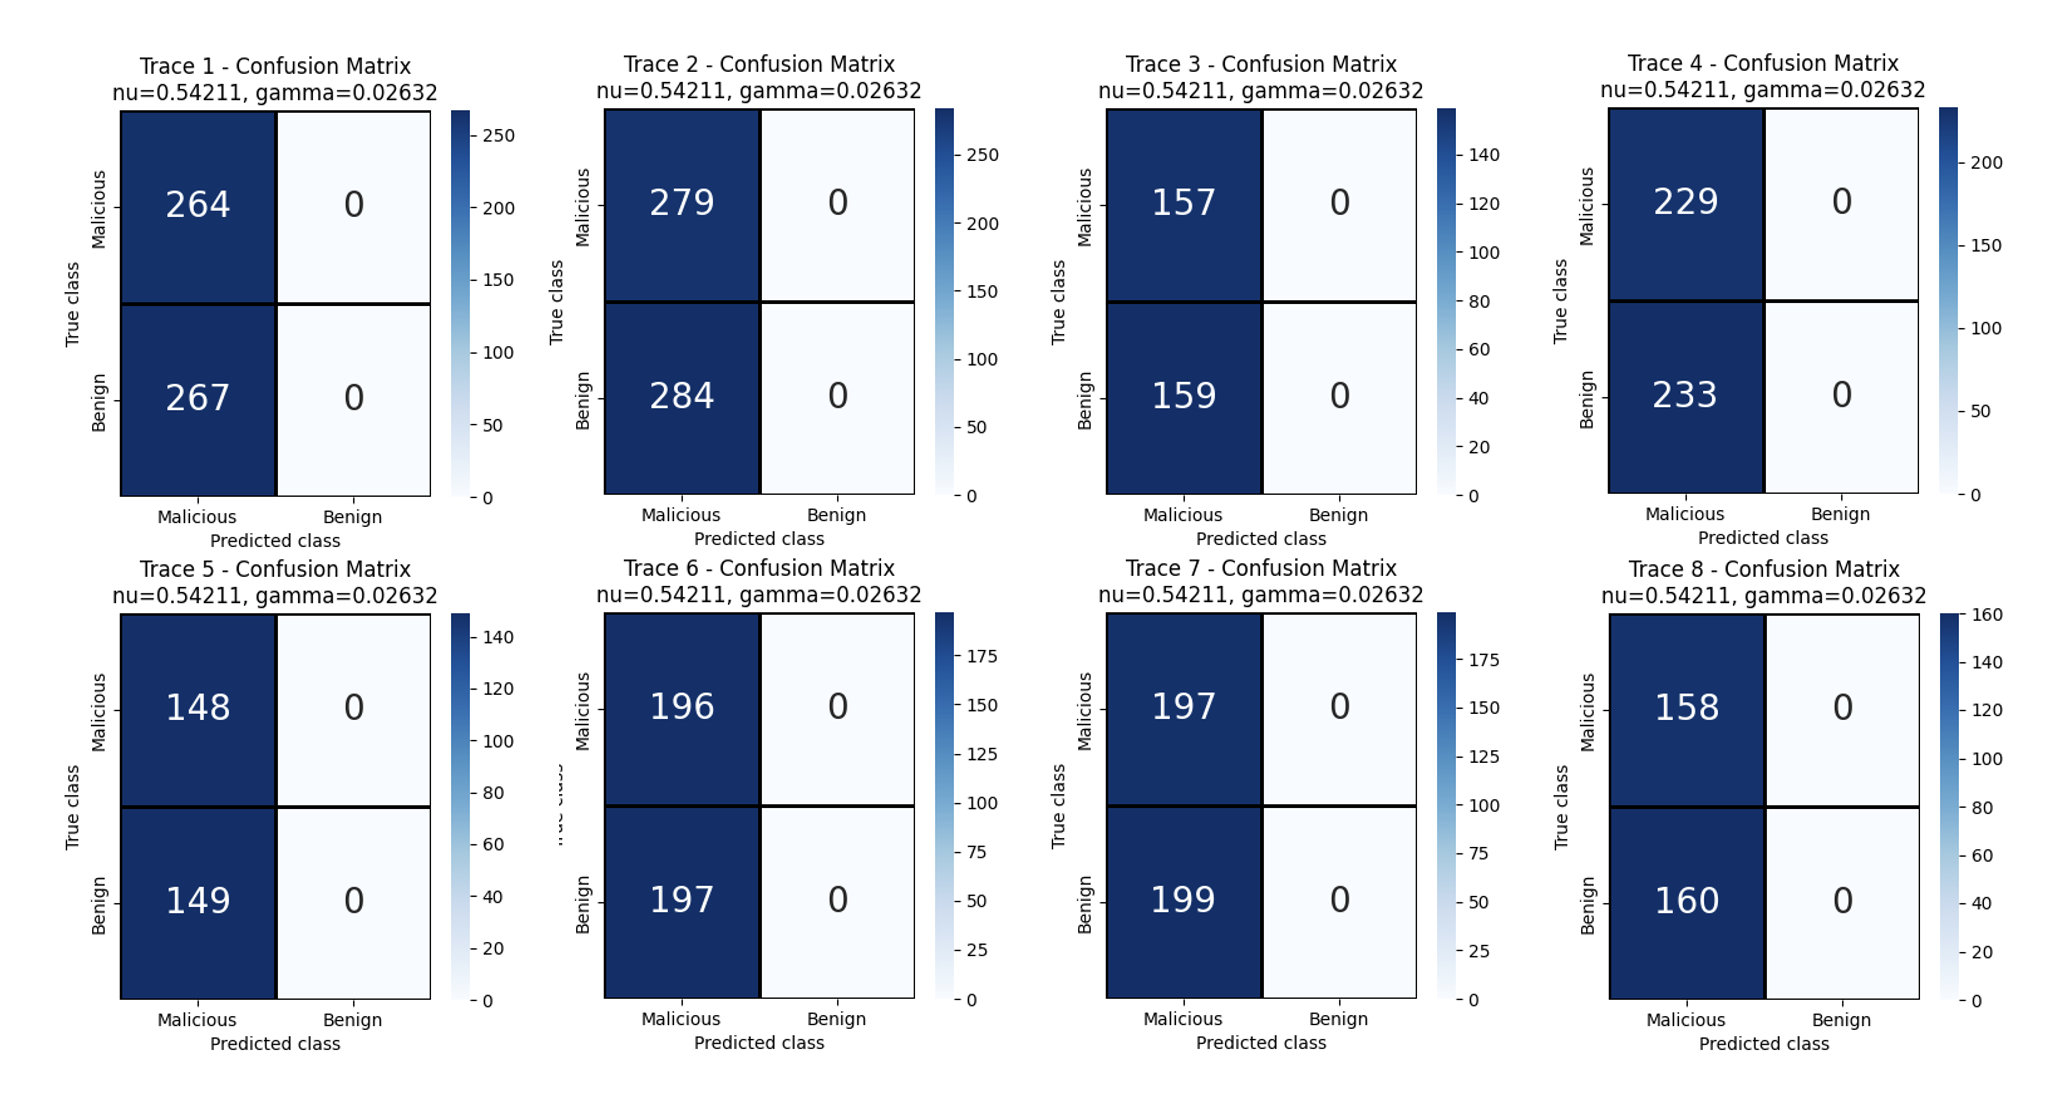
\includegraphics[width = 0.9 \linewidth]{images/ocsvm.png}
    \caption{One-Class SVM results: confusion matrices of each trace}
    \label{fig:enter-label}
\end{figure}


\end{column}

\end{columns}

    
\end{frame}
%-----------------------
\begin{frame}{Local Outlier Factors Results}

\begin{columns}

\begin{column}{0.4 \linewidth}
    \textcolor{blue}{\large{Trained on traces, tested on each trace}}
    \begin{itemize}
        \item Tuned for the optimal \(numneighbors\).

        \item Was originally the worst method in (Whelan et al. 2020) after all.

        \item Indiscriminately labels all points in the test set as malicious.

    \end{itemize}

    \vspace{5mm}
    
    \textcolor{blue}{(Whelan et al. 2020) included 85 GNSS-related and sensory data in their work.}

    \vspace{5mm}
    \textcolor{blue}{OCSVM \& LOF do not seem to generalize well on our dataset with limited status data. }
\end{column}


\begin{column}{0.7 \linewidth}
\begin{figure}
    \centering
    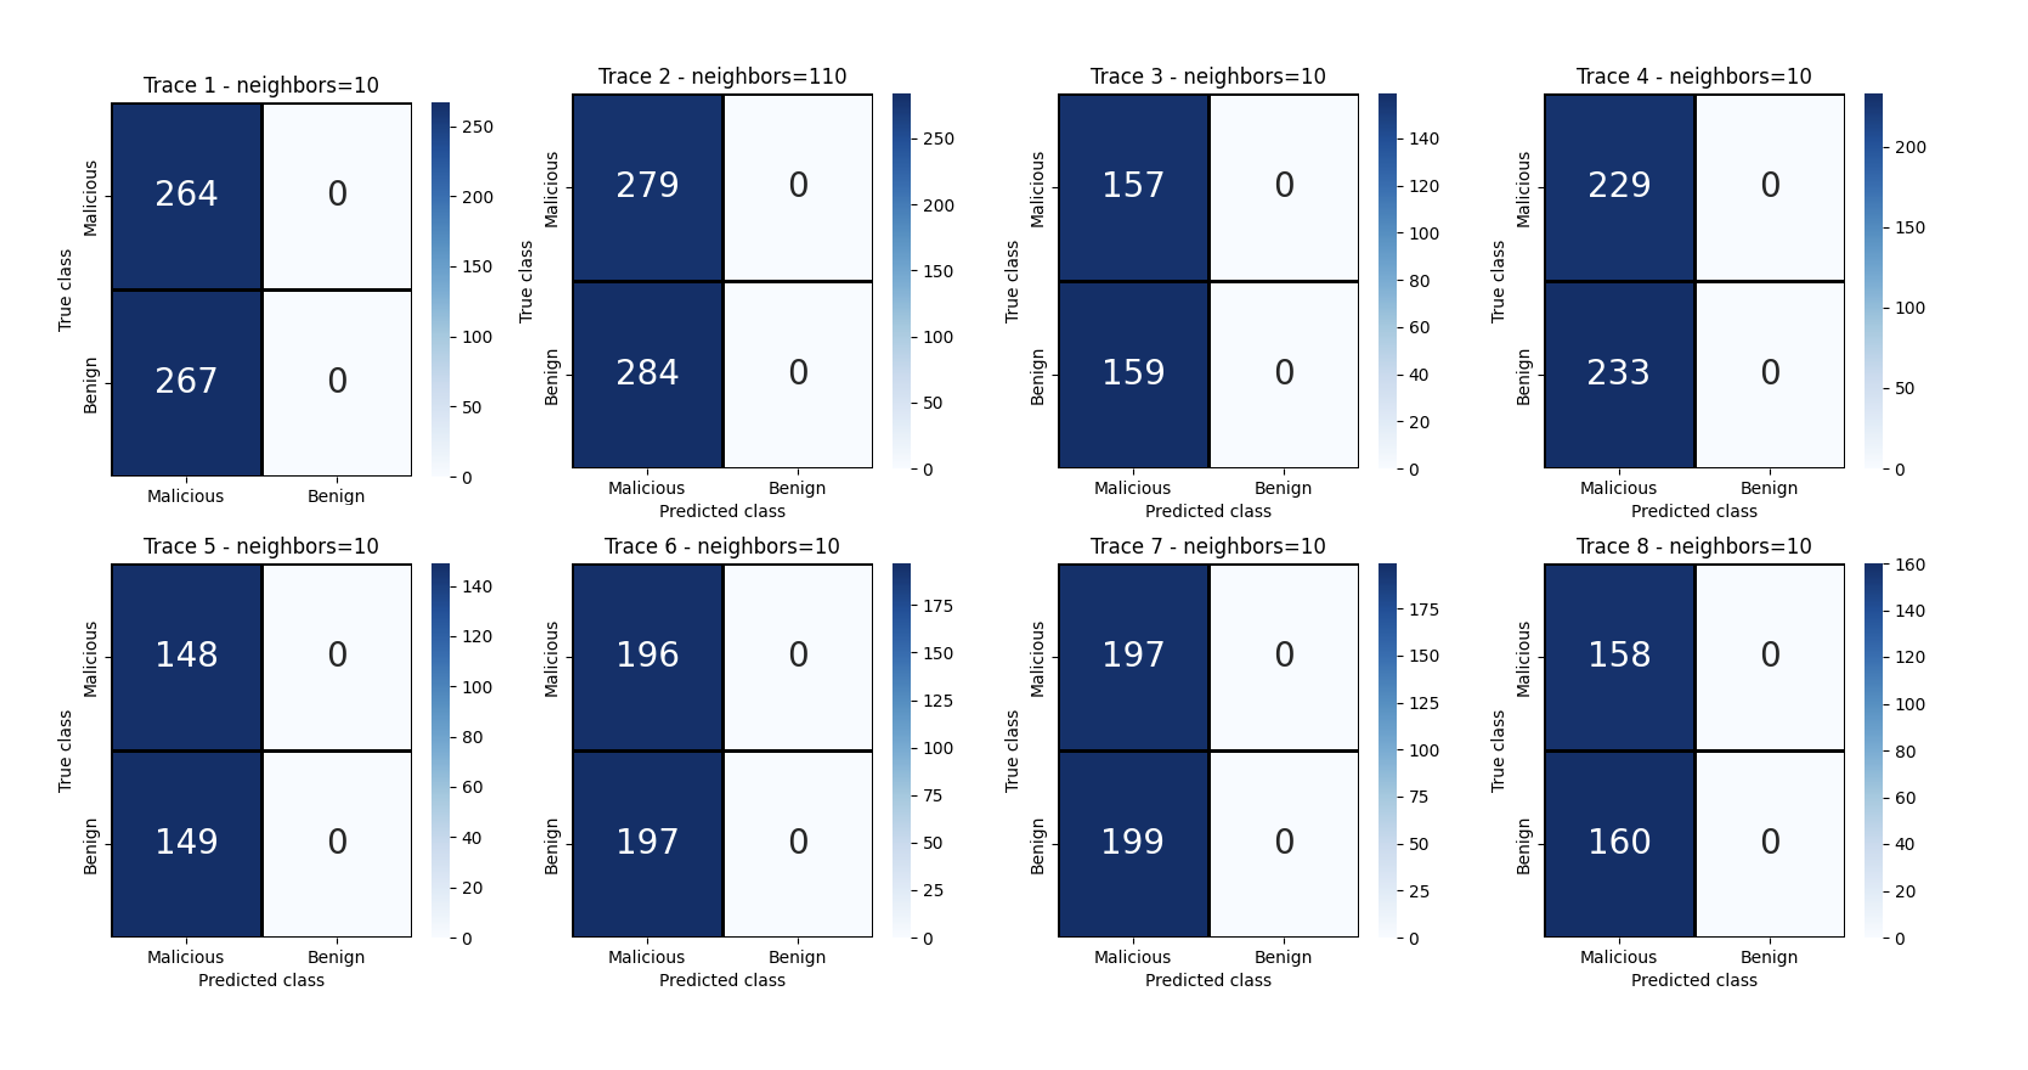
\includegraphics[width = 0.9 \linewidth]{images/lof-results.png}
    \caption{LOF results: confusion matrices of each trace}
    \label{fig:enter-label}
\end{figure}


\end{column}

\end{columns}

    
\end{frame}
%-----------------------
\begin{frame}{Autoencoder Results}


\begin{columns}

\begin{column}{0.4 \linewidth}
    {\large \textcolor{blue}{Self-defined Autoencoder Model}}
    \begin{itemize}
        \item model inputs = model ouputs
        \item Train \& validation set: The benign traces
        \item Test set for detection: The spoofed traces
        \item Hyperparameter Search
        \item Spoofed Points: MSE between outputs and inputs \(>\) predefined error threshold \(T\)
    \end{itemize}
\end{column}


\begin{column}{0.7 \linewidth}
\begin{figure}
    \centering
    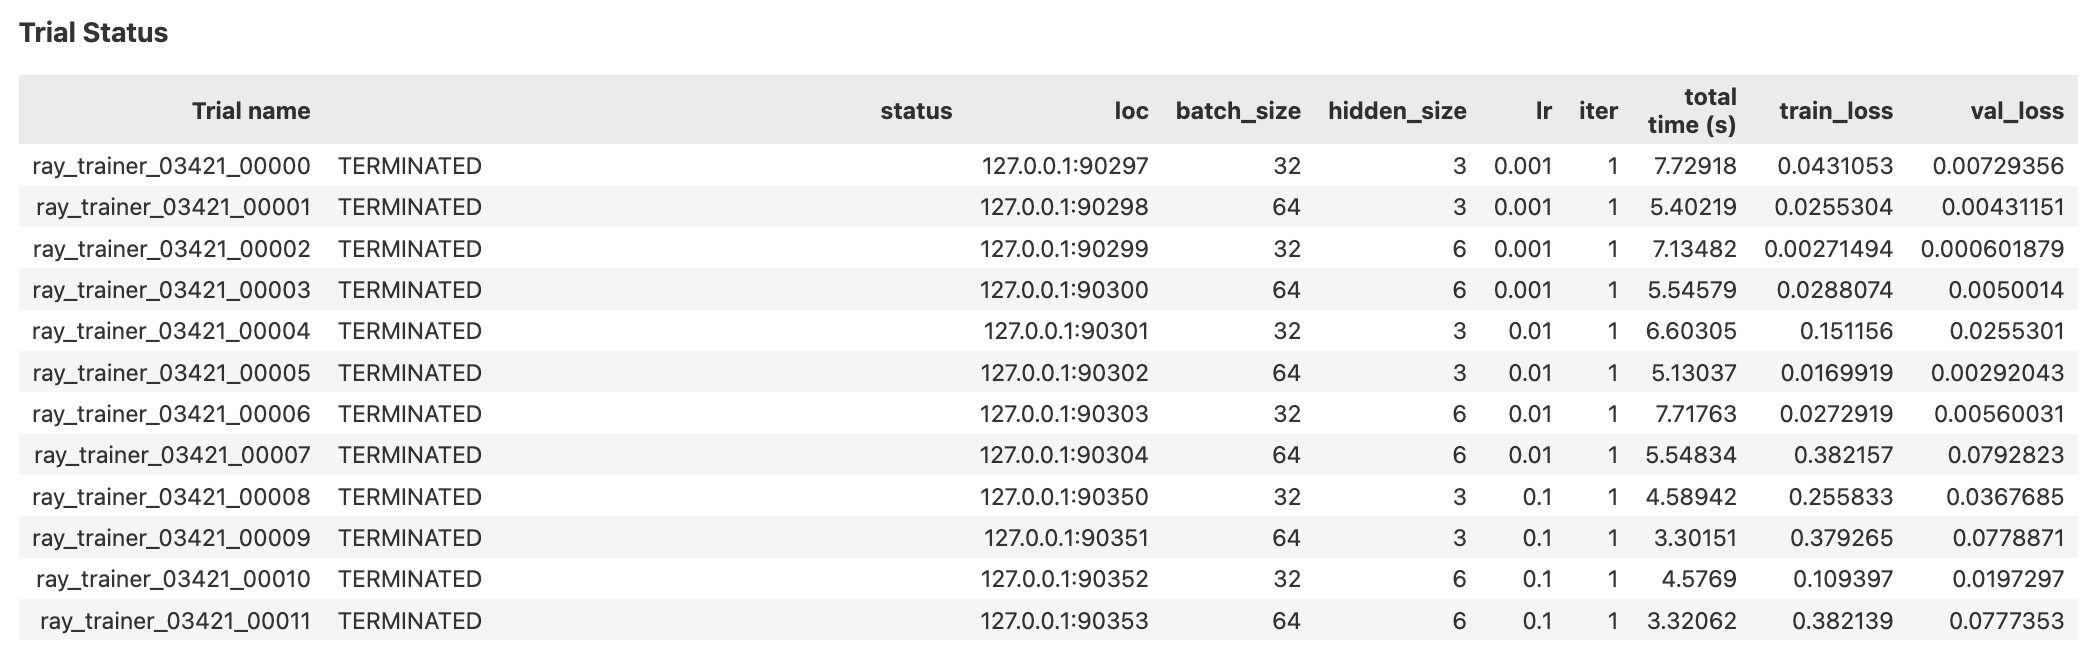
\includegraphics[width = 0.7 \linewidth]{images/ae-param-tune.png}
    \caption{Parameter Search on Autoencoder}
    \label{fig:enter-label}
\end{figure}
\begin{figure}
    \centering
    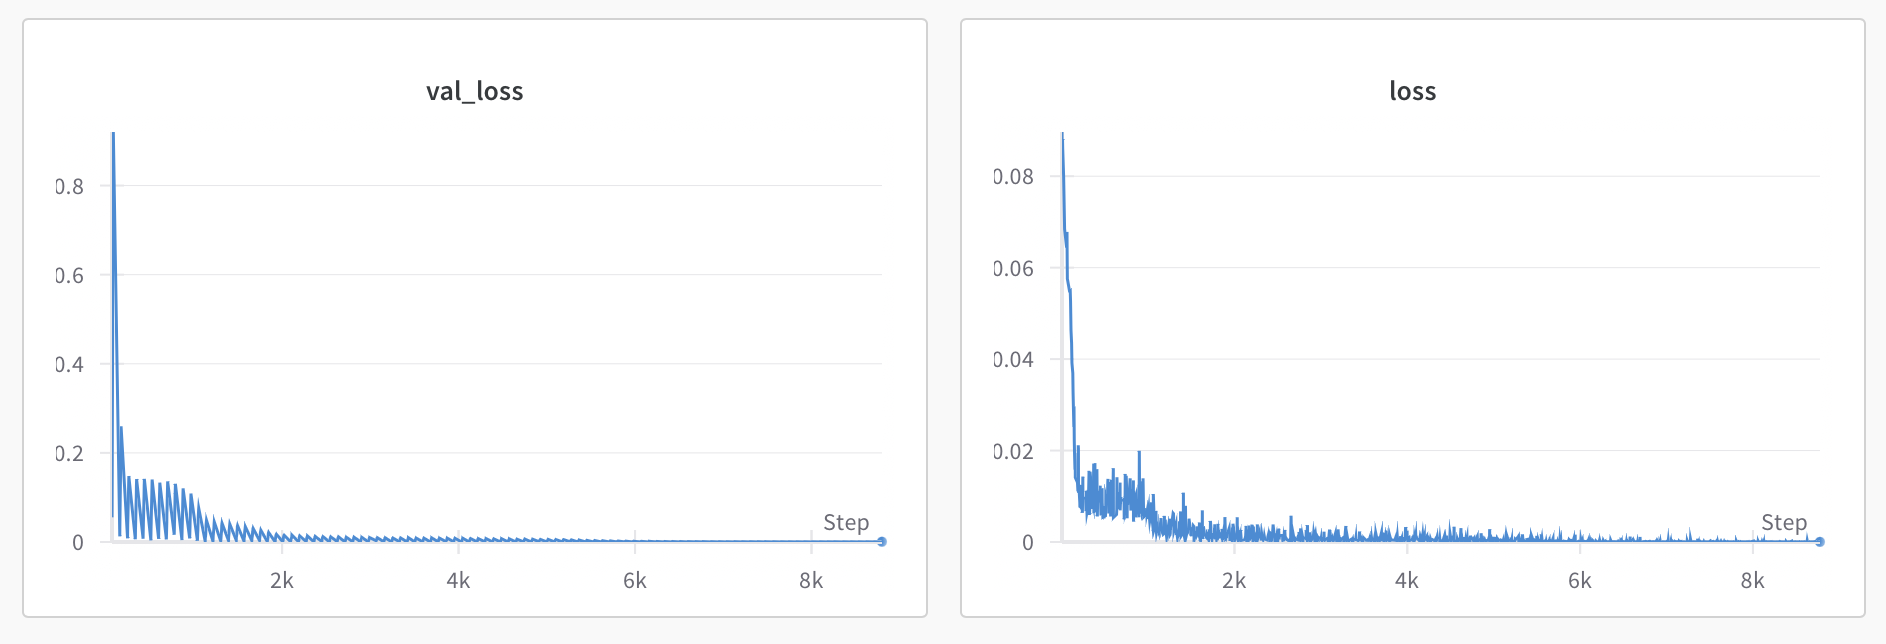
\includegraphics[width = 0.6 \linewidth]{images/ae_converge_new.png}
    \caption{Model Convergence}
    \label{fig:enter-label}
\end{figure}


\end{column}

\end{columns}

    
\end{frame}
%-----------------------
\begin{frame}{Autoencoder Results Cont'd}

\begin{columns}

\begin{column}{0.4 \linewidth}
    \textcolor{blue}{\large{Threshold \(T\) Tuning}}
    \begin{itemize}
        \item Tuning Objective.
        \begin{itemize}
            \item \(\arg\min\limits_T F_1 \text{ score}\)
        \end{itemize}
        \item Whelan et al. did not disclose how to choose the Threshold \(T\).
        \item Choose the \(T\) that achieves highest avg F1 score?
        \item Should we tune on test set?
        \item Universal Threshold vs. One Threshold for each known trace?
    \end{itemize}

    \vspace{5mm}

    \textbf{Still not ideal F1 score, compared with what Whelan et al. obtained in their work (94.81\% on average).}
\end{column}


\begin{column}{0.6 \linewidth}
\begin{figure}
    \centering
    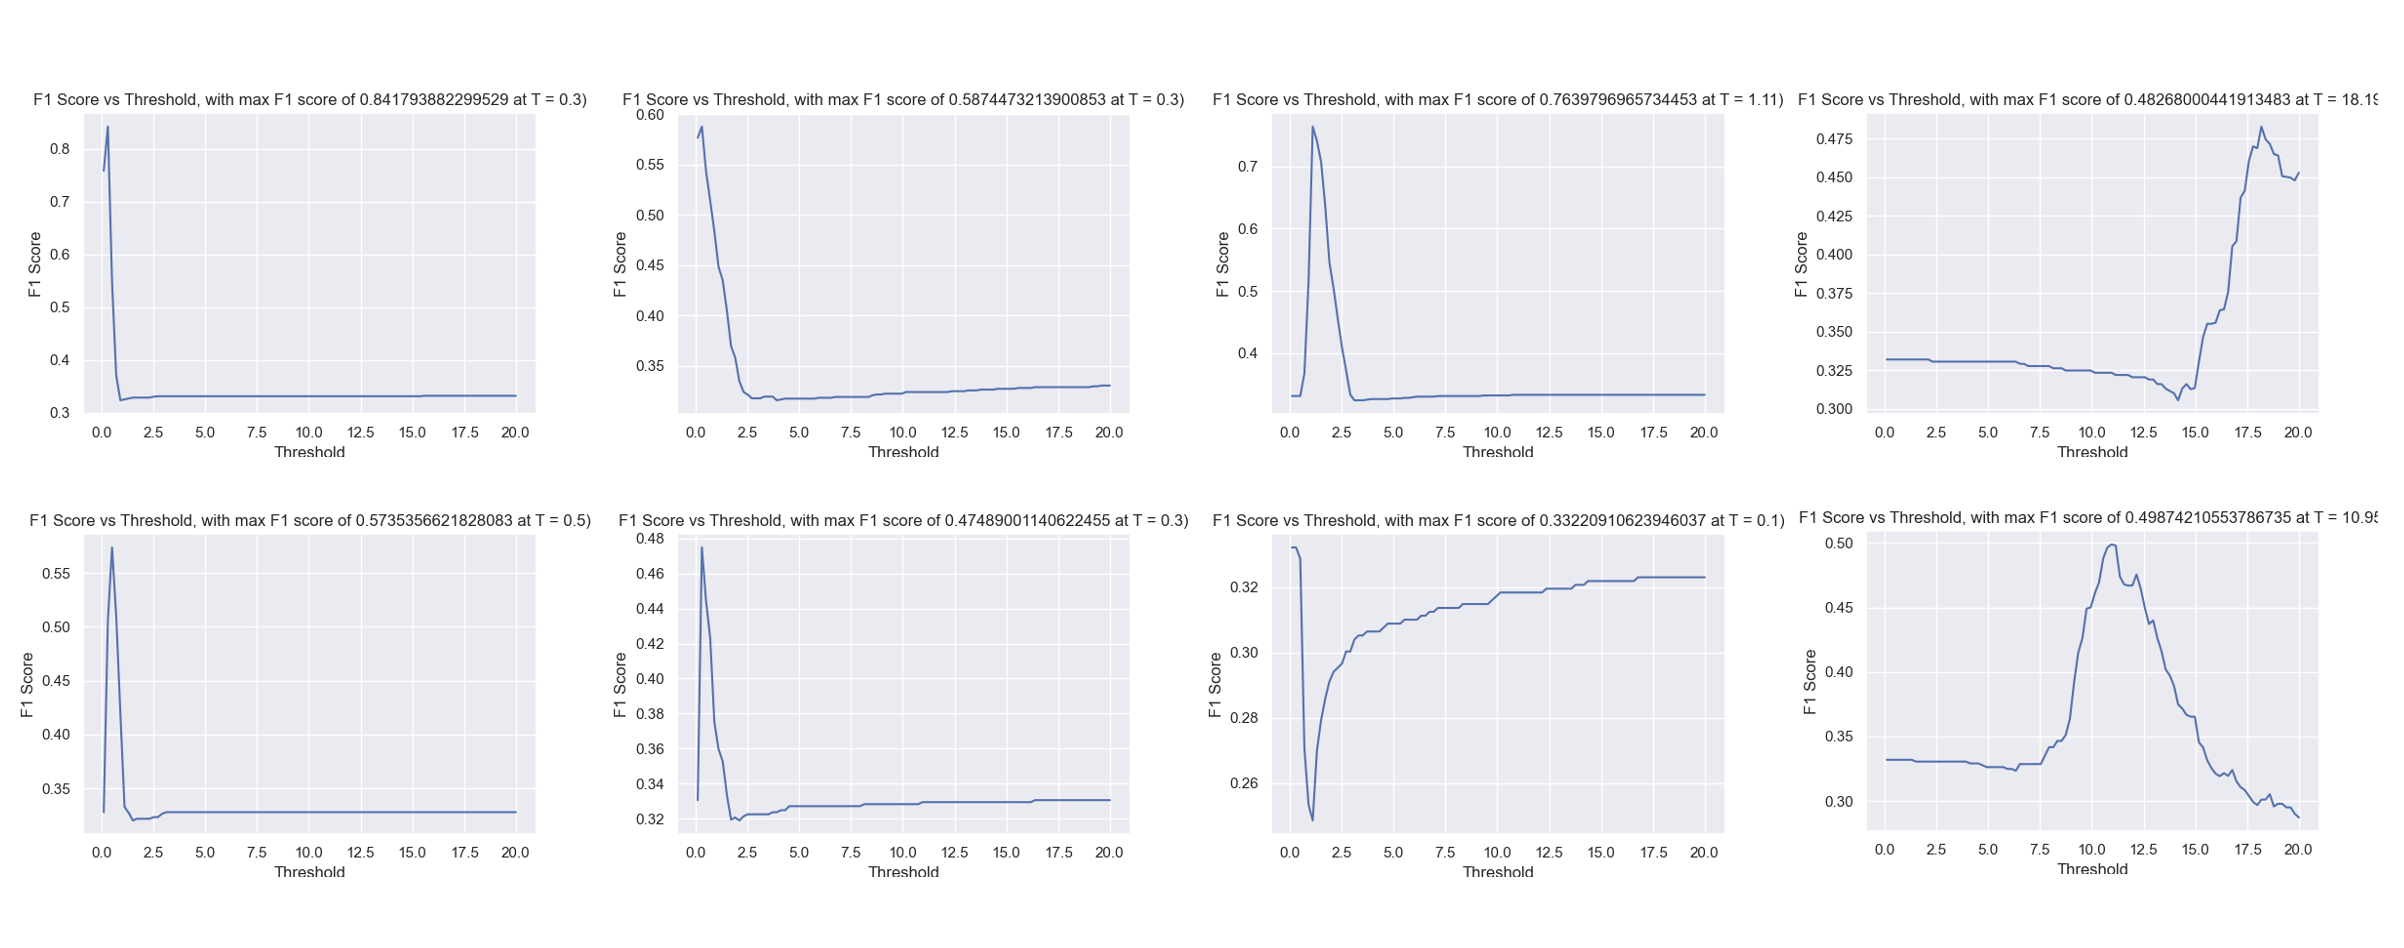
\includegraphics[width = 0.7 \linewidth]{images/ae_threshold.png}
    \caption{Tuning Threshold \(T\) w.r.t F1 score on \textcolor{blue}{each trace}}
    \label{fig:enter-label}
\end{figure}

\begin{figure}
    \centering
    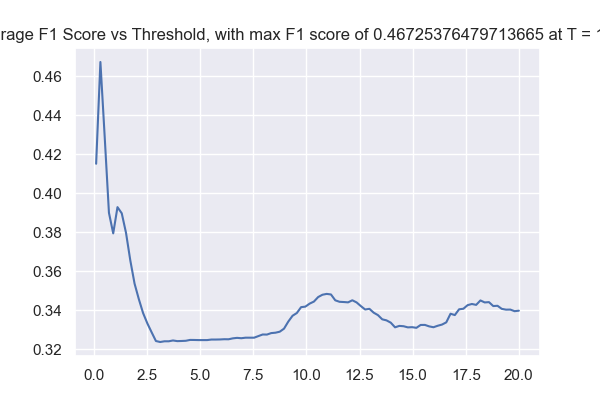
\includegraphics[width = 0.3 \linewidth]{images/avg_trace_f1.png}
    \caption{Average of F1 score on \textcolor{blue}{all traces}}
    \label{fig:enter-label}
\end{figure}
\end{column}

\end{columns}





    
\end{frame}
%-----------------------
\begin{frame}{Comparison of Three One-Class Classifiers}

    % Please add the following required packages to your document preamble:% Please add the following required packages to your document preamble:
% \usepackage{multirow}
% \usepackage{graphicx}
\begin{table}[]
\resizebox{\textwidth}{!}{%
\begin{tabular}{l|lllll}
                        & label     & precision & recall & F1 score & Hyperparameters                                    \\ \hline
\multirow{3}{*}{OC-SVM} & benign    & n/a       & n/a    & n/a      & \multirow{3}{*}{nu = 0.5421, gamma = 0.0263}       \\
                        & malicious & 0.4968    & 1.0000    & 0.6638   &                                                    \\
                        & macro avg & 0.2484    & 0.5000 & 0.3319   &                                                    \\ \hline
\multirow{3}{*}{LOF}    & benign    & n/a       & n/a    & n/a      & \multirow{3}{*}{numneighbor varies per test trace} \\
                        & malicious & 0.4968    & 1.0000    & 0.6638   &                                                    \\
                        & macro avg & 0.2484    & 0.5000 & 0.3319   &                                                    \\ \hline
\multirow{3}{*}{Autoencoder} &
  \multirow{3}{*}{macro avg} &
  \multirow{3}{*}{0.6428} &
  \multirow{3}{*}{0.6050} &
  \multirow{3}{*}{0.4808} &
  \multirow{3}{*}{tuned via paramter search} \\
                        &           &           &        &          &                                                    \\
                        &           &           &        &          &                                                   
\end{tabular}%
}
\end{table}

\end{frame}
%-----------------------




%------------------------------------------------

\subsection{Model-based Method (Garrett \& Gerdes, 2020)}
\begin{frame}{Two Methods from Garrett \& Gerdes}


\begin{columns}[T]

    \begin{column}{0.6\linewidth}

        {\small
        \begin{block}{Datasets}
            \begin{itemize}
            \item The same as that of GSM-based approach.\\
                Y\_est: position estimated by mobile cellular network.\\
                X\_GPS: position received by the GPS (real signal and our generated spoof signal).\\
            \item Detect the errors (haversine distance) between the estimated and the actual position in statistic methods.
            \end{itemize}
        \end{block}
        }
        \begin{figure}
            \centering
            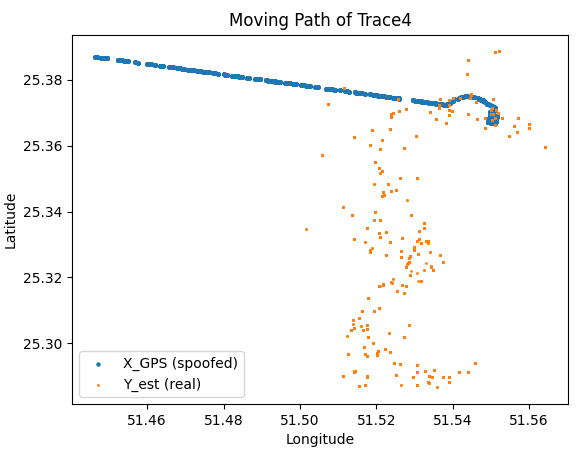
\includegraphics[width = 0.6\textwidth]{images/trace4.png}
            \label{fig:enter-label}
        \end{figure}
    \end{column}
    
    \begin{column}{0.45\linewidth}
        \begin{figure}
                \centering
                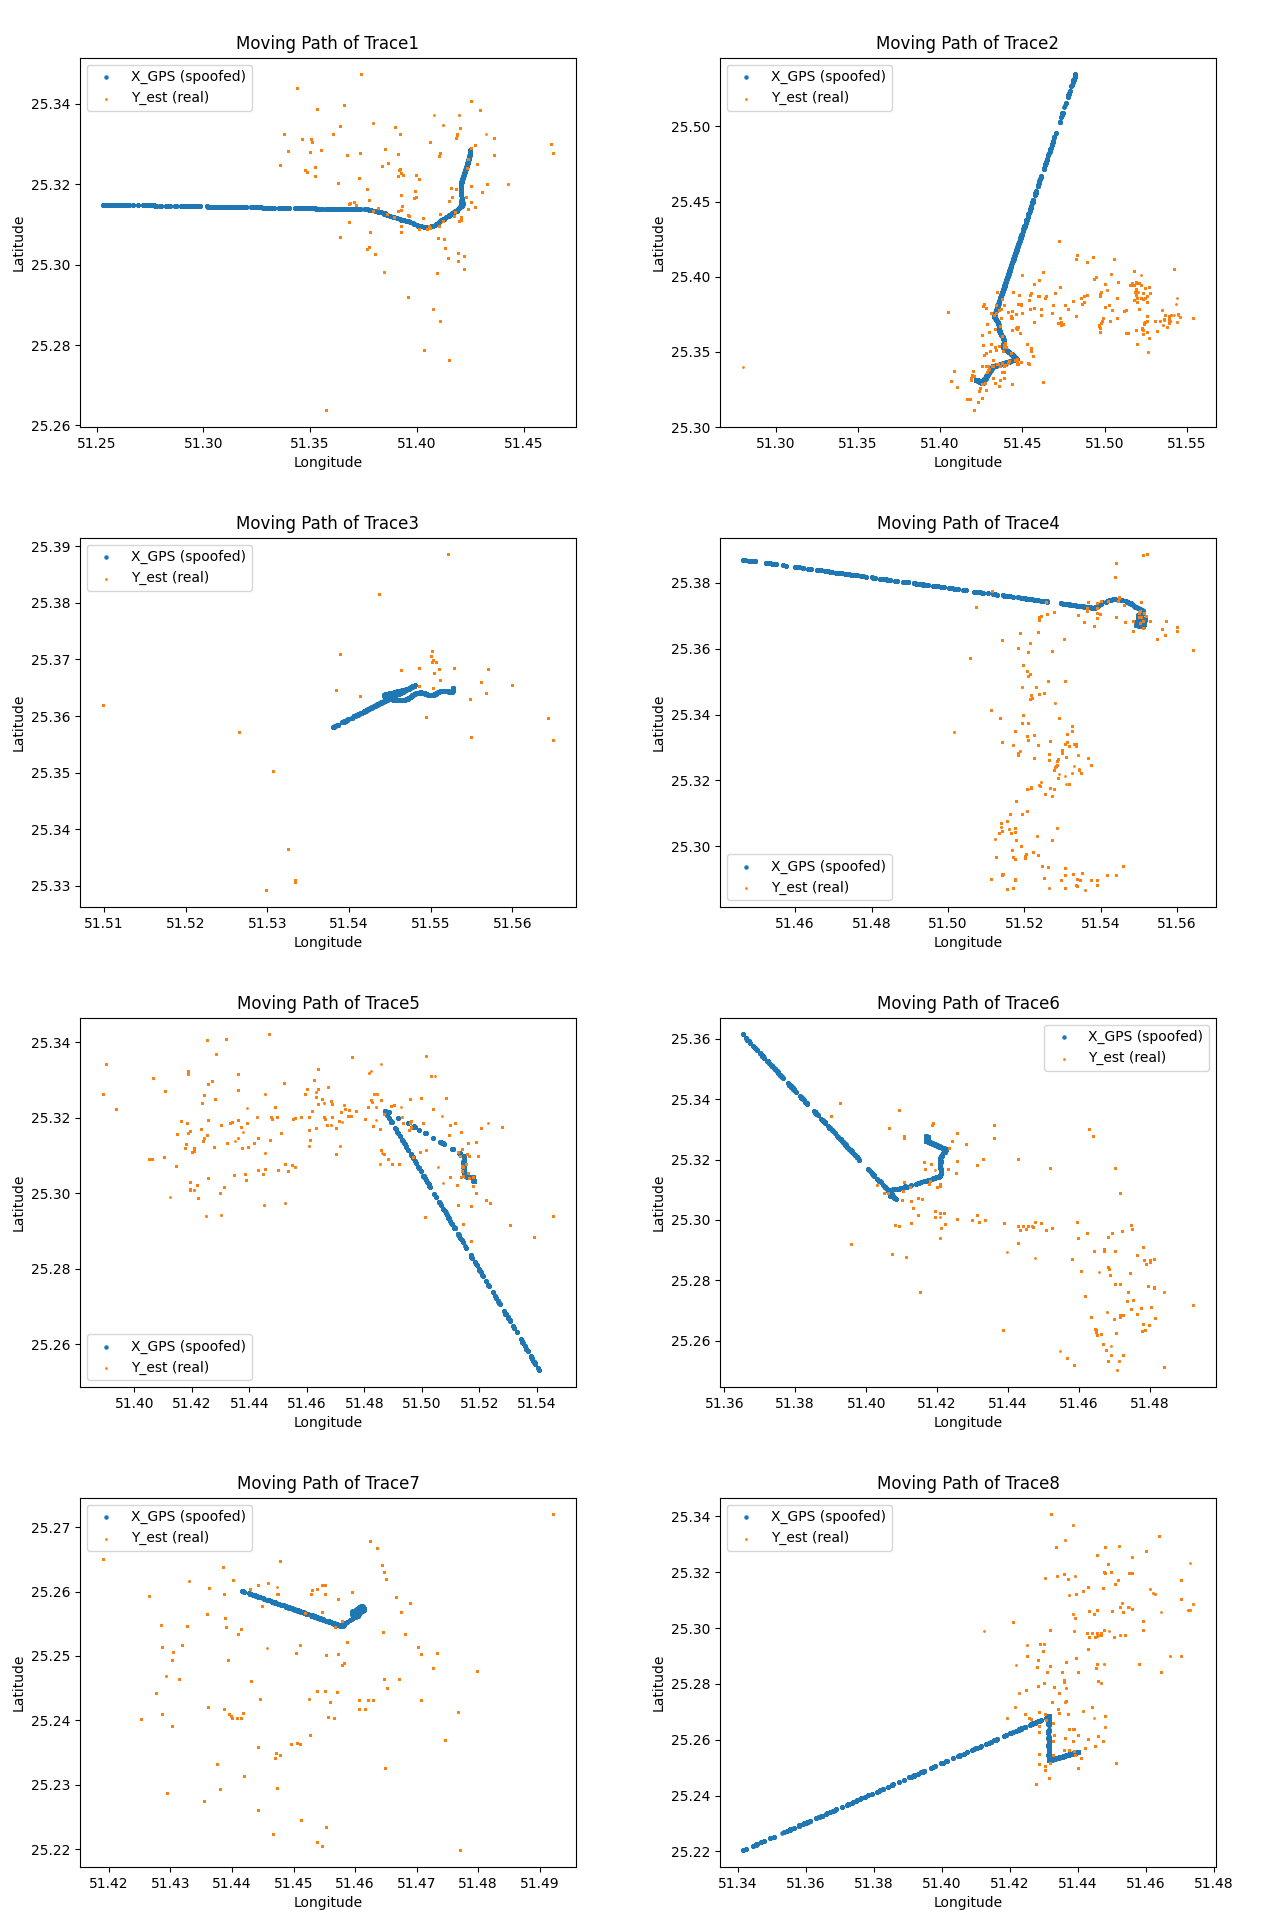
\includegraphics[width = 0.7\textwidth]{images/Garrett_moving_path.png}
                \label{fig:enter-label}
        \end{figure}
    \end{column}
\end{columns}

\end{frame}

%------------------------------------------------

\begin{frame}


\begin{columns}[T]

    \begin{column}{0.5\linewidth}
    
        \begin{block}{Threshold Method (Garrett \& Gerdes, 2020)}
            \begin{itemize}
                \item Idea: Alarm when the error exceeds the threshold continuously for more than burst length.
                \begin{itemize}
                    \item $r_t$: error (haversine distance).\\
                    \item $\tau_t$: threshold.\\
                \end{itemize}
                \item Tradeoff between FP rate and detection time.
            \end{itemize}
        \end{block}

        \begin{figure}
            \centering
            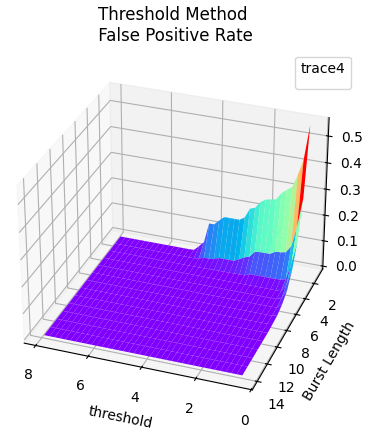
\includegraphics[width = 0.6\textwidth]{images/Garrett_FP_rate.png}
            \label{fig:enter-label}
        \end{figure}        
        
    \end{column}
    
    \begin{column}{0.5\linewidth}
        \begin{figure}
            \centering
            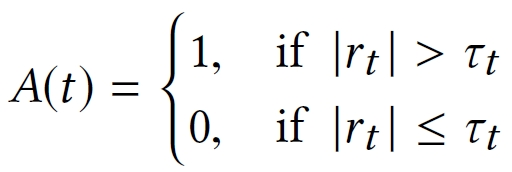
\includegraphics[width = 0.5\textwidth]{images/threshold_formula.png}
            \caption{Formula of Threshold Method}
            \label{fig:enter-label}
        \end{figure}
        \begin{figure}
            \centering
            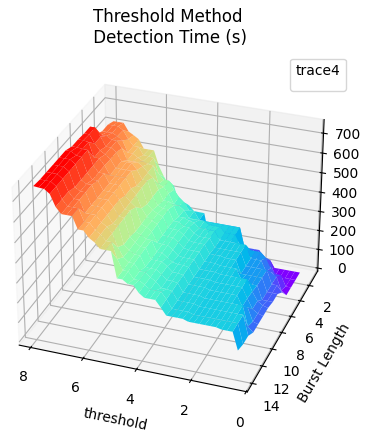
\includegraphics[width = 0.6\textwidth]{images/Garrett_detection_time.png}
            \label{fig:enter-label}
        \end{figure}
    \end{column}
\end{columns}

\end{frame}

\begin{frame}

\begin{columns}[T]

    \begin{column}{0.5\linewidth}
    
        \begin{block}{CUSUM Method (Garrett \& Gerdes, 2020)}
            \begin{itemize}
                \item Idea: Accumulate the error with a weight subtracted in each round. Once the accumulated error exceeds the threshold, trigger an alarm.
                \begin{itemize}
                    \item $S_t$: accumulated error. $\tau_t$: threshold. \\
                    \item $r_t$: error. $b_t$: weight subtracted in each round.\\
                \end{itemize}
                 \item Tradeoff between FP rate and detection time.
            \end{itemize}
        \end{block}

        \begin{figure}
            \centering
            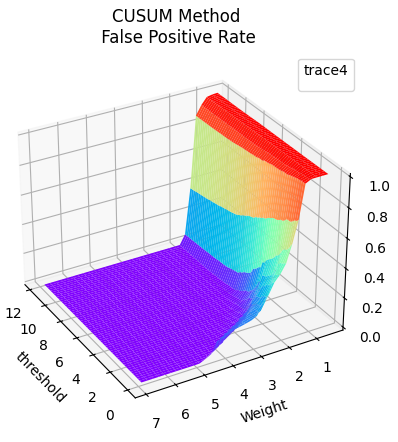
\includegraphics[width = 0.6\textwidth]{images/Garrett_FP_rate_CUSUM.png}
            \label{fig:enter-label}
        \end{figure}        
        
    \end{column}
    
    \begin{column}{0.5\linewidth}
        \begin{figure}
            \centering
            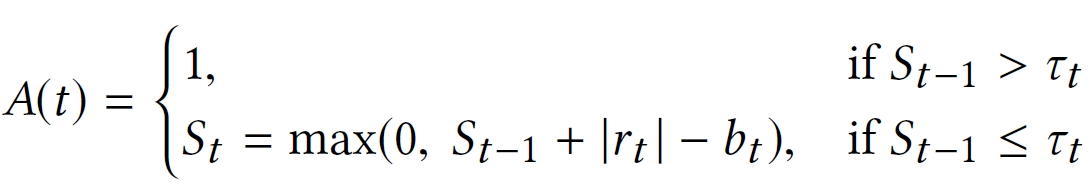
\includegraphics[width = 1.05\textwidth]{images/CUSUM_formula.png}            \caption{Formula of CUSUM Method}
            \label{fig:enter-label}
        \end{figure}
        \begin{figure}
            \centering
            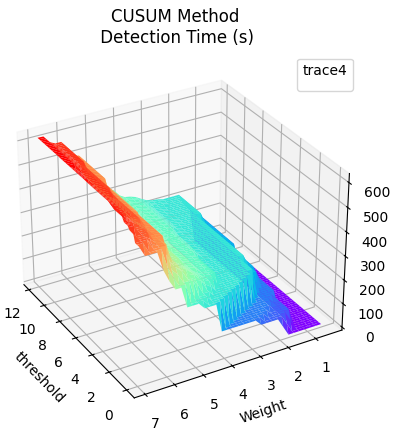
\includegraphics[width = 0.65\textwidth]{images/Garrett_detection_time_CUSUM.png}
            \label{fig:enter-label}
        \end{figure}
    \end{column}
\end{columns}

\end{frame}


\begin{frame}

\begin{columns}[T]

    \begin{column}{0.5\linewidth}
    
        \begin{block}{Tradeoff}
            \begin{itemize}
                \item Idea: Compute the arithmetic mean of FP rate and (normalized) detection time. Select the minimum point.
            \end{itemize}
        \end{block}

        \begin{figure}
            \centering
            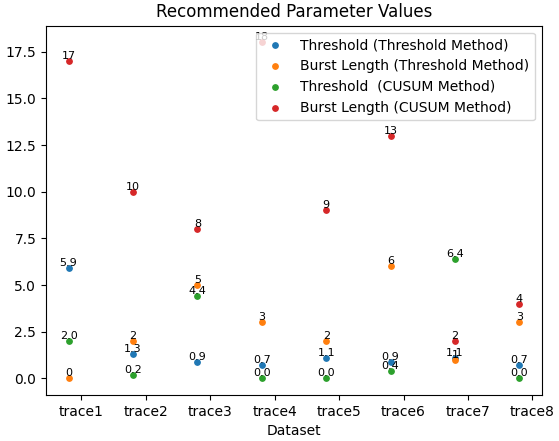
\includegraphics[width = \textwidth]{images/Recommended_Values.png}
            \label{fig:enter-label}
        \end{figure}        
        
    \end{column}
    
    \begin{column}{0.5\linewidth}
        \begin{figure}
            \centering
            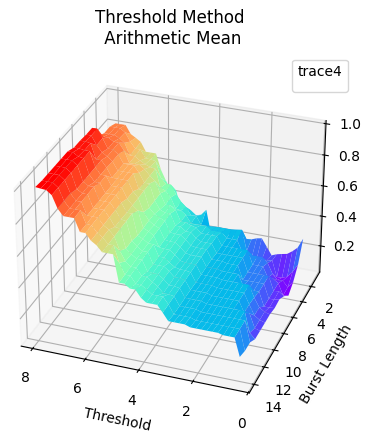
\includegraphics[width = 0.45\textwidth]{images/Garrett_arithmetic_mean.png}            
            \label{fig:enter-label}
        \end{figure}
        \begin{figure}
            \centering
            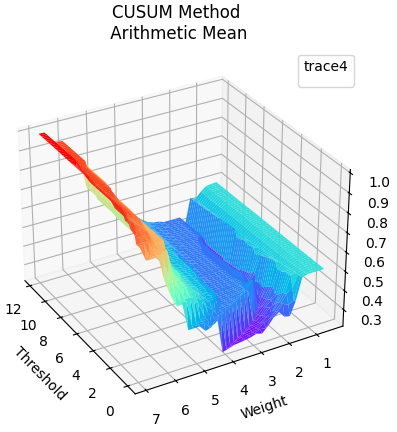
\includegraphics[width = 0.45\textwidth]{images/Garrett_CUSUM_arithmetic_mean.png}
            \label{fig:enter-label}
        \end{figure}
    \end{column}
\end{columns}

\end{frame}

\begin{frame}

\begin{columns}[T]

    \begin{column}{0.5\linewidth}
    
        \begin{block}{Result and Discussion}
            \begin{itemize}
                \item Test other datasets using the recommended parameter values on trace4.
                \item Tradeoff between FP rate and detection time.
                \item The pattern may change depending on the choice of parameter values.
            \end{itemize}
        \end{block}

        \begin{figure}
            \centering
            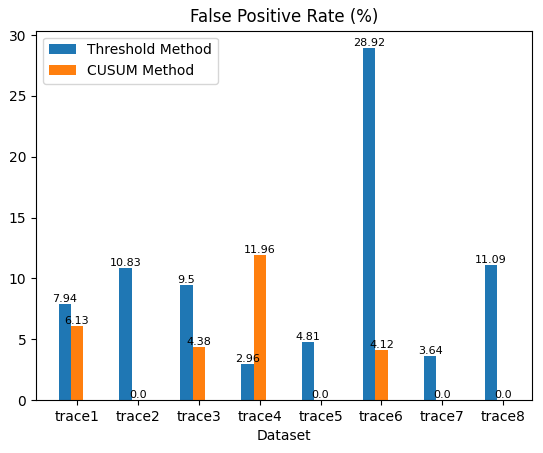
\includegraphics[width = 0.8\textwidth]{images/FP_rate.png}
            \label{fig:enter-label}
        \end{figure}        
        
    \end{column}
    
    \begin{column}{0.5\linewidth}
        \begin{figure}
            \centering
            
\includegraphics[width = 0.8\textwidth]{images/detection_time.png}
            \label{fig:enter-label}
        \end{figure}
    \begin{block}{Compared with Other ML Methods}
            \begin{itemize}
                \item Lightweight, fast, not require many data.
                \item Suitable for small drones.
                \item Parameters need to be adjusted according to the actual situation.
            \end{itemize}
        \end{block}
        
    \end{column}
\end{columns}

\end{frame}
%------------------------------------------------


\section{Discussion}

\subsection{Performance Analysis}
\begin{frame}{Comparison of Model Performance}

% Please add the following required packages to your document preamble:
% \usepackage{graphicx}
% \usepackage[table,xcdraw]{xcolor}
% Beamer presentation requires \usepackage{colortbl} instead of \usepackage[table,xcdraw]{xcolor}
\begin{table}[]
\resizebox{\textwidth}{!}{%
\begin{tabular}{l|llll}
\rowcolor[HTML]{EFEFEF} 
                              & GSM                      & PCA+One-class Classifier & Threshold Method (Garret et al.) & CUSUM (Garret et al.) \\ \hline
\textbf{Performance Metrics}                 &                          &                          &                                  &                       \\
\rowcolor[HTML]{EFEFEF} 
F1 Score &
  \begin{tabular}[c]{@{}l@{}}N/A \\ benign sequences \\ \(\gg\) attack sequence\end{tabular} &
  \begin{tabular}[c]{@{}l@{}}46\%\\  (Autoencoder, \\average of all traces)\end{tabular} &
  \begin{tabular}[c]{@{}l@{}}N/A \\ (TP is not applicable)\end{tabular} &
  \begin{tabular}[c]{@{}l@{}}N/A \\ (TP is not applicable)\end{tabular} \\
False Positive Rate &
  \begin{tabular}[c]{@{}l@{}}10.5\%\\  (on test set)\end{tabular} &
  \begin{tabular}[c]{@{}l@{}}34.69\%\\  (Autotencoder on trace 4)\end{tabular} &
  \begin{tabular}[c]{@{}l@{}}9.1\% \\ (on trace 4)\end{tabular} &
  \begin{tabular}[c]{@{}l@{}}0.0\% \\ (on trace 4)\end{tabular} \\
\rowcolor[HTML]{EFEFEF} 
Detection Rate &
  \begin{tabular}[c]{@{}l@{}}8/8\\ (on all traces)\end{tabular} &
  \begin{tabular}[c]{@{}l@{}}8/8\\ (on all traces)\end{tabular} &
  \begin{tabular}[c]{@{}l@{}}8/8\\ (on all traces)\end{tabular} &
  \begin{tabular}[c]{@{}l@{}}8/8\\ (on all traces)\end{tabular} \\
Detection Time (Quantitative) & 98.330s on train dataset & 0.0437s (trace 4)        & 0.3s (on trace 4)                & 173.2s (on trace 4)   \\
\rowcolor[HTML]{EFEFEF} 
Detection Time (Qualitative)  & Relatively Slow          & Very fast                & Very fast                        & Slow                 
\end{tabular}%
}
\end{table}
* 

\end{frame}

%------------------------------------------------

\subsection{Comparison of Models Used}
\begin{frame}{Comparison of Model Algorithms}

% Please add the following required packages to your document preamble:
% \usepackage{graphicx}
% \usepackage[table,xcdraw]{xcolor}
% Beamer presentation requires \usepackage{colortbl} instead of \usepackage[table,xcdraw]{xcolor}
\begin{table}[]
\resizebox{\textwidth}{!}{%
\begin{tabular}{l|ll}
                           & GSM                                      & PCA+One-class Classifier           \\ \hline
\rowcolor[HTML]{EFEFEF} 
\textbf{Algorithm-related Aspects} &                                          &                                    \\
Unit of Model Prediction   & Sequence                                 & Single points in one trace         \\
\rowcolor[HTML]{EFEFEF} 
Unit of Detection          & Trace, FP rate = P(spoofed)              & Single points in one trace         \\
Deviation moment detecting & Can detect                               & Can detect under more context      \\
\rowcolor[HTML]{EFEFEF} 
Scoring measures           & Prediction anomaly sequence in one trace & Predictions of points in one trace \\
Cross-validation           & Applicable                               & Applicable                         \\
\rowcolor[HTML]{EFEFEF} 
Threshold Tuning &
  \begin{tabular}[c]{@{}l@{}}Needed for evaluating \\ the anomaly sequence\end{tabular} &
  \begin{tabular}[c]{@{}l@{}}Needed for Autoencoder\\ Not needed for LOF/OCSVM\end{tabular}
\end{tabular}%
}
\end{table}



%  table 2

% Please add the following required packages to your document preamble:
% \usepackage{graphicx}
% \usepackage[table,xcdraw]{xcolor}
% Beamer presentation requires \usepackage{colortbl} instead of \usepackage[table,xcdraw]{xcolor}
\begin{table}[]
\resizebox{\textwidth}{!}{%
\begin{tabular}{l|ll}
                           & Threshold Method (Garret et al.) & CUSUM (Garret et al.)      \\ \hline
\rowcolor[HTML]{EFEFEF} 
\textbf{Algorithm-related Aspects} &                                  &                            \\
Unit of Model Prediction   & Single points in one trace       & Single points in one trace \\
\rowcolor[HTML]{EFEFEF} 
Unit of Detection &
  \begin{tabular}[c]{@{}l@{}}Single points in one trace\\ but detection rate is based on trace unit)\end{tabular} &
  \begin{tabular}[c]{@{}l@{}}Single points in one trace\\ but detection rate is based on trace unit\end{tabular} \\
Deviation moment detecting & Can detect                       & Can detect                 \\
\rowcolor[HTML]{EFEFEF} 
Scoring measures &
  \begin{tabular}[c]{@{}l@{}}Predictions of points in one trace\\ Not applicable for confusion matrix\end{tabular} &
  \begin{tabular}[c]{@{}l@{}}Predictions of points in one trace\\ Not applicable for confusion matrix\end{tabular} \\
Cross-validation           & Applicable                       & Applicable                 \\
\rowcolor[HTML]{EFEFEF} 
Threshold Tuning &
  \begin{tabular}[c]{@{}l@{}}The drone needs to be tested in advance \\ to obtain suitable parameters.\end{tabular} &
  \begin{tabular}[c]{@{}l@{}}The drone needs to be tested in advance \\ to obtain suitable parameters.\end{tabular}
\end{tabular}%
}
\end{table}







\end{frame}

% Please add the following required packages to your document preamble:




\begin{frame}{Comparison of Scenario Settings}

% Please add the following required packages to your document preamble:
% \usepackage{graphicx}
% \usepackage[table,xcdraw]{xcolor}
% Beamer presentation requires \usepackage{colortbl} instead of \usepackage[table,xcdraw]{xcolor}
\begin{table}[]
\resizebox{\textwidth}{!}{%
\begin{tabular}{l|llll}
 &
  GSM &
  PCA+One-class Classifier &
  Threshold Method (Garret et al.) &
  CUSUM (Garret et al.) \\ \hline
\rowcolor[HTML]{EFEFEF} 
\textbf{Scenario-related Aspects} &
   &
   &
   &
   \\
\begin{tabular}[c]{@{}l@{}}Regularity \\ of Flight path\end{tabular} &
  Not Required &
  Required &
  Not Required &
  Not Required \\
\rowcolor[HTML]{EFEFEF} 
Fixed-route &
  Not Required &
  Required &
  Not Required &
  Not Required \\
Pretraining &
  Required &
  Required &
  Required &
  Required \\
\rowcolor[HTML]{EFEFEF} 
\begin{tabular}[c]{@{}l@{}}Detection \\ Effeciency\end{tabular} &
  High &
  Very high &
  Very high &
  \begin{tabular}[c]{@{}l@{}}High (worse than \\ Garrett’s Threshold Method)\end{tabular} \\
Training Time &\begin{tabular}[c]{@{}l@{}}
  very fast, O(mn) with\\  n time points, m base stations\end{tabular} &
  \begin{tabular}[c]{@{}l@{}}Converges very Fast \\ for Autoencoder\end{tabular} &
  Fast &
  Fast \\
\rowcolor[HTML]{EFEFEF} 
Comments &
  \begin{tabular}[c]{@{}l@{}}Need GSM or Wifi signal \\ together with GPS\end{tabular} &
   &
   &
  
\end{tabular}%
}
\end{table}

\end{frame}


%------------------------------------------------

\subsection{Reflection}

\begin{frame}{Why are the results not ideal?}

    \Huge{\centerline{The experiment results are not very ideal.}}
    \Huge{\centerline{What could possibly have gone wrong?}}
\end{frame}

%------------------------------------------------
\begin{frame}{Reflecting on the Selected Methods}


\begin{columns}[T]

    \begin{column}{0.5\linewidth}

        \begin{block}{GSM-Based Approach (Oligeri et al. 2019)}
        \begin{itemize}
            \item \textbf{\textcolor{blue}{RSS}} The Exponential Distribution of RSS may not be the best model .
            \item \textbf{\textcolor{blue}{Duration threshold}} The duration threshold used to determine attack may be overfitting.
            \item \textbf{\textcolor{blue}{Spoofed trace}} The generated spoofed path may not interact with real GPS signal.        
        \end{itemize}
        \end{block}
            


        \begin{block}{Novelty-Based Approach: PCA + One-Class Classifiers (Whelan et al. 2020)}
            \begin{itemize}
                \item \textbf{\textcolor{blue}{Point-wise detection}} when do we mark the starting point of spoofing? what if there are mixed ordered occurence of benign and malicoius label predictions? 
                \item \textbf{\textcolor{blue}{Threshold tuning}} Should we use test set to tune \(T\)?
            \end{itemize}
        \end{block}
    \end{column}
    
    
    \begin{column}{0.5\linewidth}
        \begin{block}{Model-Based Method (Garrett \& Gerdes, 2020)}
            \item \textbf{\textcolor{blue}{Cell sites}} Cell sites are sparse in rural areas, which can lead to poor estimates of the drone’s location.
            \item \textbf{\textcolor{blue}{Tradeoff}} Hard to tradeoff and set the optimal parameters. A configuration optimal on one path may perform poorly on another path.
        \end{block}
        \begin{figure}
            \centering
            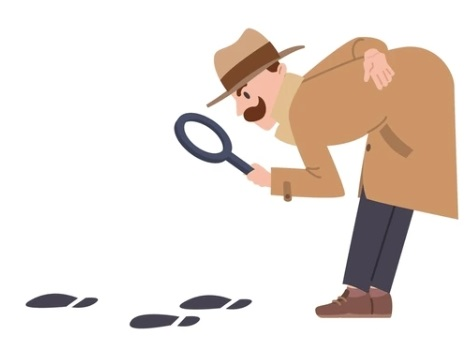
\includegraphics[width = 0.7\textwidth]{images/curious.png}
            \label{fig:enter-label}
        \end{figure}
    \end{column}
\end{columns}


    
\end{frame}




%------------------------------------------------
\begin{frame}{Reflecting on the Experiment Dataset}

\begin{columns}[T]

    \begin{column}{0.5\linewidth}
        
    \begin{block}{Dataset Availability Issue}
            \item \textbf{\textcolor{blue}{Generated sensor data}}
            
            Lack of necessary IMU sensor data for novelty based methods.
            \begin{itemize}
                \item Drastic data generation and transformation.
                \item Not good enough sensor data (obtained by differentiation). Not enough variety.
            \end{itemize}
            \item \textbf{\textcolor{blue}{Generated spoofed track}} 
            
            \begin{itemize}
                % \item Position seems to be only received from the GNSS, not own real position.
                \item \textcolor{blue}{Identifiable Spoofed Pattern} Generated spoofed traces compromise the robustness of our experiments. (Moving in a straight line simply screams "I'm spoofed")
                \item \textcolor{blue}{Simplification of Scenario} The attacker will usually monitor our position and speed to launch \textbf{a more plausible spoofing attack}.
                % \item the generated spoof path is a straight line, which doesn't interact with real GPS signals.
            \end{itemize}
            
    \end{block}
    

    \end{column}
    
    \begin{column}{0.5\linewidth}
     \begin{figure}
         \centering
         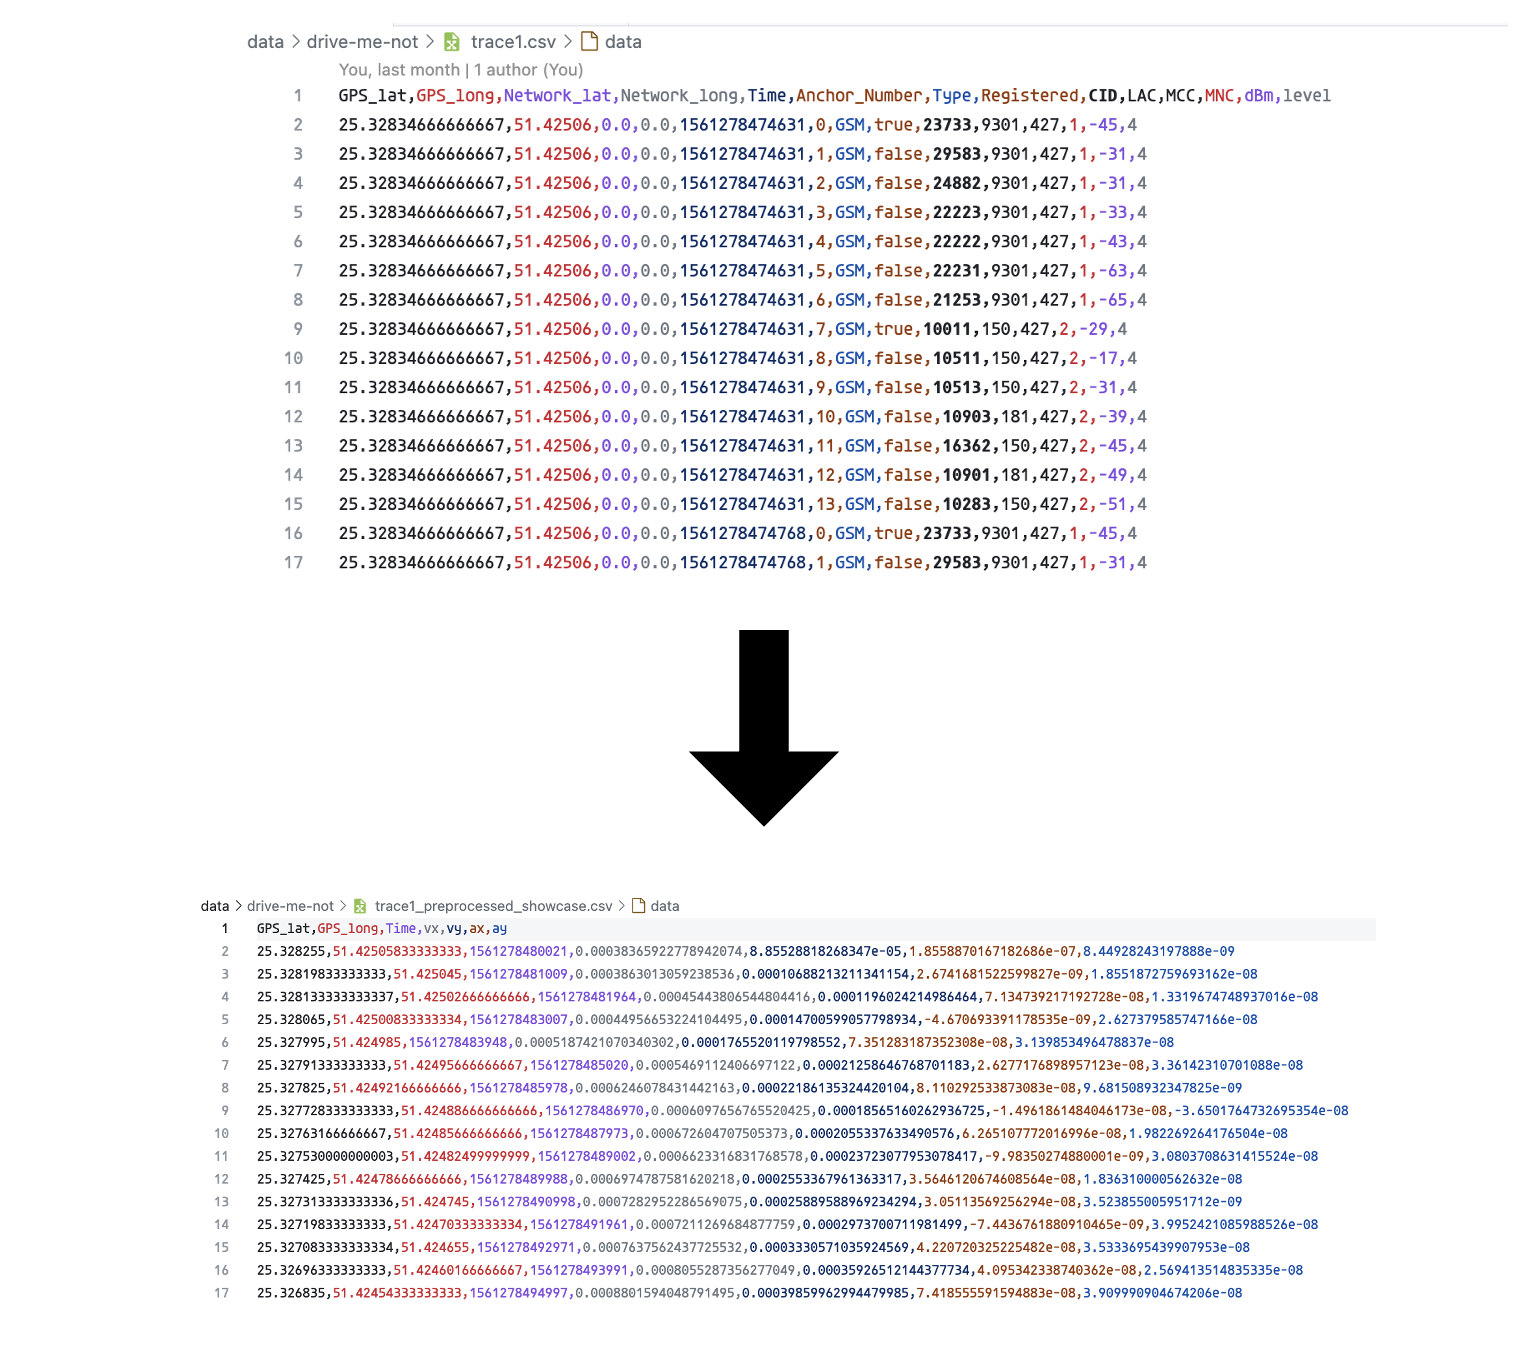
\includegraphics[width = \linewidth]{images/data-ge.png}
         \caption{Drastic data generation and transformation}
         \label{fig:enter-label}
     \end{figure}
    \end{column}
\end{columns}

\end{frame}

%------------------------------------------------




%------------------------------------------------

\subsection{Future Research}
\begin{frame}{Future Improvements}

\large
\begin{itemize}
    \item \textbf{Comprehensive Dataset for Comparison (Research Question of Group 5)} Comprehensive datasets that could be applied to  most papers to compare their performance
    % \item 
\end{itemize}
    
\end{frame}

%------------------------------------------------

% \begin{frame}[fragile] % Need to use the fragile option when verbatim is used in the slide
% \frametitle{Citation}
% An example of the \verb|\cite| command to cite within the presentation:\\~

% This statement requires citation \cite{p1}.
% \end{frame}

% %------------------------------------------------

% \begin{frame}
% \frametitle{References}
% \footnotesize{
% \begin{thebibliography}{99} % Beamer does not support BibTeX so references must be inserted manually as below
% \bibitem[Smith, 2012]{p1} John Smith (2012)
% \newblock Title of the publication
% \newblock \emph{Journal Name} 12(3), 45 -- 678.
% \end{thebibliography}
% }
% \end{frame}

%------------------------------------------------


\begin{frame}
\Huge{\centerline{Q \& A}}
\end{frame}

%----------------------------------------------------------------------------------------

\end{document}